\documentclass{article} % change ``USenglish'' to ``norsk'' if applicable.
\usepackage{preamble}

%% To easily include matlab code, I would recommend to have a look at this answer https://tex.stackexchange.com/a/158816 which has nice examples.

%% It uses: https://ctan.org/pkg/matlab-prettifier

\begin{document}

% Titlepage
\title{LaTeX Lab Report Skeleton}
\author{Group ??\\Vemund Rogne\\Jørgen Haaland}
\date{January 1, 1970}
\begin{titlepage}
    \maketitle
    \begin{figure}
    \centering
    
\includegraphics[width=0.5\textwidth]{figures/itk_ntnu}\\
    Department of Engineering Cybernetics
    \end{figure}
    \thispagestyle{empty}
\end{titlepage}

% TOC
\newpage
\tableofcontents
\thispagestyle{empty} % Avoid page numbering on the table of contents.


% Main content
\newpage
\setcounter{page}{1}
\include{evaluation_info} % <--- delete/comment this before handing in the final PDF!
\documentclass[../main.tex]{subfiles}

\begin{document}

\section{Optimal Control of Pitch/Travel without Feedback}\label{kap:Part2OptimalControlWithoutFeedback}

\subsection{Derivation of a continous time state space model}
In this part of the exercise we will disregard elevation, therefore we assume $ e = 0 $ and do include it in the model.

The state-vector, $\bm x$ is defined as:
\begin{equation}\label{eq:lab2_state}
	\bm x = 
	\begin{bmatrix}
		\lambda & r & p & \dot p
	\end{bmatrix}
	^T ,
\end{equation}
where $\lambda$ is travel, $r$ is the travel rate, $p$ is pitch and $\dot{p}$ is pitch rate.

The dynamic equations for the system was given in the problem description \todo{Add ref to page and paper}. These following equations were given:
\begin{subequations} \label{eq:lab2_states_eq}
	\begin{align}
		\dot \lambda &= r \\
		\dot r &= -K_2 p, \quad K_2 = \frac{K_p l_a}{J_t}\\
		\dot p &= \dot p \\
		\ddot p &= -K_1 V_d = K_1 K_{pd} \dot p - K_1 K_{pp} p + K_1 K_{pp} pc, \quad K_1 = \frac{K_f l_h}{J_p}
	\end{align}
\end{subequations}
The state-space form of the system therefore becomes: 
\begin{equation}\label{eq:lab2_cont_ss}
	\underbrace{\begin{bmatrix}
		\dot \lambda \\
		\dot r \\
		\dot p \\
		\ddot p
	\end{bmatrix}}_{\bm{\dot x}} = 
	\underbrace{
	\begin{bmatrix}
		0 & 1 & 0 & 0 \\
		0 & 0 & -K_2 & 0 \\
		0 & 0 & 0 & 1 \\
		0 & 0 & -K_1 K_{pp} &  -K_1 K_{pd}
	\end{bmatrix}
	}_{\bm A_c}
	\begin{bmatrix}
		\lambda \\ r \\ p \\ \dot{p} \\
	\end{bmatrix}
	+
	\underbrace{
		\begin{bmatrix}
			0 \\ 0 \\ 0 \\ K_1 K_{pp}
		\end{bmatrix}
	}_{\bm B_c} \underbrace{p_c}_{u}
\end{equation}

\subsubsection{A deeper dive into the state-space model}
The state-space form of the system models two part of the whole system, namely: 
\begin{enumerate}
	\item The physics of the helicopter.
	\item The proportional-derivative controller for the pitch.
\end{enumerate}
This is shown in \cref{fig:lab2_system} where the red dotted box shows what we model with the state space model. \todo[inline]{Add ref to the figure in the problem description}

\begin{figure}[h]
	\centering
	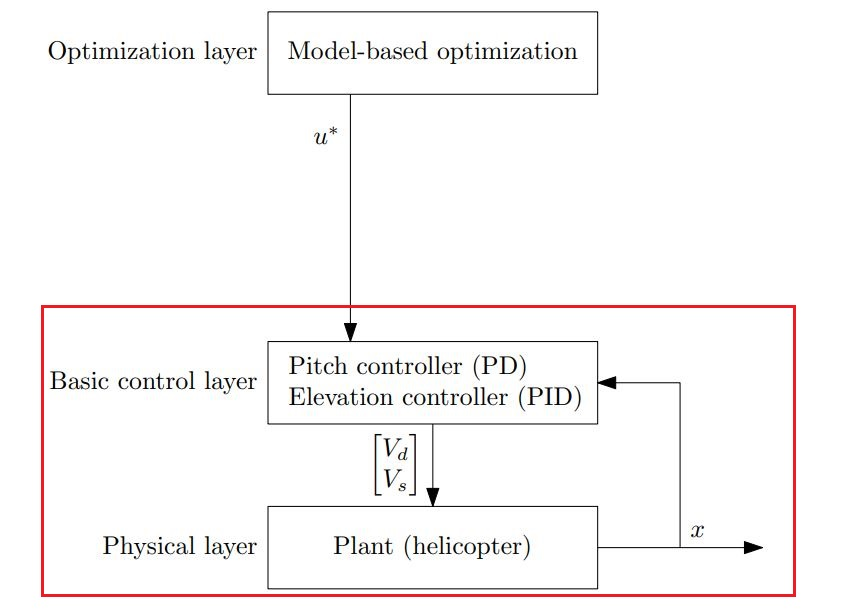
\includegraphics[width=0.8\linewidth]{figures/lab2_system}
	\caption{The red box encapsulate what is modelled in the state space model described by \cref{eq:lab2_cont_ss}.}
	\label{fig:lab2_system}
\end{figure}

This becomes clear studying the equations in \cref{eq:lab2_states_eq}. They describe the helicopters physics for all states except elevation and elevation rate. $ \lambda $ and $ r $ is dependent on the helicopters pitch, $ p $. $ p $ and $ \dot p  $ is however dependent on the voltage difference, $ V_d $. The voltage difference is the output of the PD-controller for controlling the pitch\todo{Should we add acronym list?}. 

To summarize, this means that our state space model describes the helicopter's physics through the dynamic equations for $ \lambda $, $ r $, $ p $ and $ \dot p $, while the equation of $ V_d $ describes the PD-controller used to control the pitch angle. In total our state-space model is modelling both the helicopter and the PD controller for pitch.


\subsubsection{Stability and eigenvalues}
The properties of this system is dependent on physical constants ($l_a, J_t, ...$) and control parameters ($K_{pp}, K_{pd}$).

Symbolic expressions in Matlab shows that the eigenvalues of A are:
\begin{equation}
	\lambda = \pm \frac{1}{2} \left( \sqrt{-K_1 (-K_1 K_{pd}^2 + 4  K_{pp})} - K_1  K_{pd} \right)
\end{equation}

The eigenvalues of the continous model, with $K_{pp} = 0,1 , K_{pd} = 0,4$ are:
\begin{equation}\label{eq:lab2_ss_c_eigenvalues_example}
	\begin{bmatrix}
		0 \\ 0 \\ -0.26 + 0.24i \\ -0.26 - 0.24 \\
	\end{bmatrix}
\end{equation}

% ------------------- DISCRETIZING THE MODEL ------------------------
\subsection{Discretizing the continous time model} \label{sec:lab2_disc}
A discretized model is required for generating an optimal trajectory. \textit{[...] continous time models require quite different solution methods} \cite{FossHeirung}

We will discretize the model using the forward Euler method, which is given by:
\todo[inline]{Do we need to derive forward euler?}
\begin{equation}\label{eq:lab2_forward_euler}
	\bm{x}[k + 1] = \bm I \bm x[k] + T\bm{A_c x}[k] + T\bm B_c ,
\end{equation}
where $ T $ is the sample-time in the discrete model.\todo
[inline]{Add reference to linsys slides}
Reformulating this, we can write:
\begin{equation}\label{eq:lab2_discrete_system}
	\bm{x}_{k + 1} = \underbrace{(\bm I + T \bm A_c)}_{\bm A_d} \bm{x}_{k} + \underbrace{T \bm B_c}_{\bm B_d} u_k
\end{equation}
On matrix form $ \bm A_d $ and $ \bm B_d $ becomes: 
\begin{equation}
	\bm A_d = \begin{bmatrix}
		1 & T & 0 & 0 \\
		0 & 1 & -T K_2 & 0 \\
		0 & 0 & 1 & T \\
		0 & 0 & -T K_1 K_{pp} &  1 - T K_1 K_{pd}
	\end{bmatrix}, \quad 
	\bm B_d = \begin{bmatrix}
		0 \\ 0 \\ 0 \\T K_1 K_{pp}
	\end{bmatrix}
\end{equation}




\subsubsection{Checking stability}
The stability condition for \cref{eq:lab2_discrete_system} is that all eigenvalues of $ \bm A_d $ is less than one in absolute values, i.e.:
\begin{equation}\label{eq:lab2_stab_condition}
	|\lambda_i| \leq 1, \quad \text{for } i = 1, 2, 3, 4
\end{equation}, where $ \lambda_i $ is the i'th eigenvalue of $ \bm A_d $.

Using the script in \cref{lst:lab2_eigenvalues} the eigenvalues became:
\begin{subequations}\label{eq:lab2_eigenvalues}
	\begin{align}
		\lambda_1 &= 1 \\
		\lambda_2 &= 1 \\
		\lambda_3 &= 0.55 \\
		\lambda_4 &= 0.55
	\end{align}
\end{subequations}
All eigenvalues fulfills the requirement of \cref{eq:lab2_stab_condition}, which means our system is stable! Since two of the eigenvalues are on the unit circle (i.e. has a value of 1), our system is more specifically marginally stable. More information on this subject can be found \todo{Add cite to wikipedia}.

\lstinputlisting[caption= {MATLAB code for calculating eigenvalues for $ \bm A_d $}, label = {lst:lab2_eigenvalues}, language=Matlab]{code/calculate_eigenvals.m}

\subsection{The open loop optimization problem}
% https://ntnu.blackboard.com/ultra/courses/_24653_1/cl/outline
%where $q$ is the weight of input-usage. Subject to constraints.
The open loop optimization problem is a constrained quadratic program that can be solved using the Matlab function quadprog. The quadprog function requires the input to be in standard form:

\begin{equation}\label{eq:lab2_quadprog_std_form}
	\min_x \frac{1}{2} \bm x^t \bm H \bm x + \bm f^T \bm x \quad \text{such that} \begin{cases}
		\bm A \bm x \leq \bm b, \\
		\bm A_{eq} \bm x = \bm B_{eq}, \\
		\bm{lb} \leq \bm x \leq \bm{ub}		
	\end{cases}
\end{equation}

The next subsections describes this process.

\subsubsection{Formulating the cost function} \label{sec:lab2_cost_func}
As the problem description states, the cost function used in this exercise is:
\begin{equation} \label{eq:lab2_start_cost_func}
	\phi = \sum_{i=0}^{N-1} \left( \lambda_{i+1} - \lambda_f \right)^2 + qp_{ci}^2 , \quad q \ge 0
\end{equation}

Which can be rewritten with $ \bm x $ and $ u $:
\begin{equation}\label{eq:lab2_start_cost_func_2}
	f(\bm x, u) = \sum_{i=0}^{N-1} \left( \bm x_{i+1} - \bm x_f \right)^T \bm Q \left( \bm x_{i+1} - \bm x_f \right) + q u^2
\end{equation}
where
\begin{equation}\label{eq:lab2_lambda_f}
	\bm x_f = \begin{bmatrix}
		\lambda_f \\ 0 \\ 0 \\ 0
	\end{bmatrix}
\end{equation}
\begin{equation}\label{eq:lab2_Q}
	\bm Q = \begin{bmatrix}
		1 & 0 & 0 & 0 \\
		0 & 0 & 0 & 0 \\
		0 & 0 & 0 & 0 \\
		0 & 0 & 0 & 0
	\end{bmatrix}
\end{equation}
In this case we have that $ \lambda_f = 0 $ and therefore $ \bm x_f = \bm 0 $, and \cref{eq:lab2_start_cost_func_2} can be rewritten as:

\begin{equation}\label{eq:lab2_LQR}
	f(\bm x, u) = \sum_{i=0}^{N-1} \bm x_{i+1}^T \bm Q \bm x_{i+1} + r u^2
\end{equation}
where
\begin{equation}\label{eq:lab2_R}
	r = q
\end{equation}

Defining the the $z$ vector as:
\begin{equation}\label{eq:lab2_z}
	\bm z = \begin{bmatrix}
		\bm x_1 & \bm x_2 & ... & \bm x_n & u_0 & u_1 &... & u_{n-1} 
	\end{bmatrix}^T
\end{equation}
we can rewrite summation form in \cref{eq:lab2_LQR} to matrix-form:
\begin{equation}\label{eq:lab2_quadprog}
	f(\bm z) = \bm z^T \bm H \bm z
\end{equation}
with
\begin{equation}\label{eq:lab2_H}
	\bm H = \begin{bmatrix}
		\bm Q & 0 & \cdots  & 0 & 0 & 0 & \cdots & 0\\
		0 & \bm Q & \cdots  & 0 & 0 & 0 & \cdots & 0\\
		 & & \ddots &  &  &  &  & \\
		0 & 0 & \cdots & \bm Q & 0 & 0  & \cdots & 0\\
		0 & 0 & \cdots & 0 & r & 0  & \cdots & 0\\
		0 & 0 & \cdots & 0 & 0 & r  & \cdots & 0\\
		 & &  &  &  &  & \ddots & \\
		0 & 0 & \cdots & 0 & 0 & 0  & \cdots & r
	\end{bmatrix}
\end{equation}


\subsubsection{The constraints of the optimization problem} \label{sec:lab2_constraints}
There are two separate types of constrains in this problem, the system itself and imposed constraints. The system constrains is described by the physics of the helicopter, which we have modeled in \cref{eq:lab2_discrete_system}. Imposed constraints are constraints added by the designer of the system. 

In this case we have an imposed constraint on the pitch given by:
\begin{equation}
	\left\lvert p_k \right\rvert \le \frac{30}{180} \pi, k \in \left\{ 1, ..., N \right\} 
\end{equation}
As the manipulated variable $ p_c $ is the setpoint for the $ p $ controller, this constraint must also be implemented for the setpoint. Since there is no inequality constraints on the other states, they have lower bounds of $ -\infty $ and upper bounds of $ \infty $. This gives us the inequality constraints for the state and the input as: 
\begin{subequations}
	\begin{align}
		\bm x^{low} = \begin{bmatrix}-\infty \\ -\infty \\ -\frac{30}{180} \pi \\ -\infty \end{bmatrix} &\leq \bm x \leq \bm x^{high} = \begin{bmatrix} \infty \\ \infty \\ \frac{30}{180} \pi \\ \infty \end{bmatrix} \\
		u^{low} = -\frac{30}{180} \pi &\leq u \leq u^{high} = -\frac{30}{180} \pi
	\end{align}
\end{subequations}
We can now easily expand this to define lower- and upper-bounds for the vector $ \bm z $ given in \cref{eq:lab2_z}
\begin{equation}\label{eq:lab2_z_bounds}
		\bm z^{low} = \begin{bmatrix}
			\bm x^{low}\\
			\vdots \\
			\bm x^{low}\\
			u^{low}\\
			\vdots \\
			u^{low}
		\end{bmatrix} \leq \bm z \leq
		\bm z^{high} = \begin{bmatrix}
			\bm x^{high}\\
			\vdots\\
			\bm x^{high}\\
			u^{high}\\
			\vdots \\
			u^{high}\\
		\end{bmatrix}
\end{equation}



The system constraints can be defined as: 
\begin{equation}\label{eq:lab2_physical_constraints}
	\bm A_{eq} \bm z = \bm b_{eq}
\end{equation}
, where
%The physics of the helicopter is added in $A_{eq}$ and $b_{eq}$.
\begin{equation} \label{eq:lab2_Aeq_beq}
	\bm A_{eq} = 
	\begin{bmatrix}
		\bm I & 0 & \cdots & \cdots & 0 & -\bm B_d & 0 & \cdots & \cdots & 0 \\
		-\bm A_d & \bm I & \ddots & & \vdots & 0 & \ddots & \ddots & & \vdots \\
		\vdots && \ddots & \ddots & 0 & \vdots & & \ddots & \ddots & 0 \\
		0 & \cdots & 0 & -\bm A_d & \bm I & 0 & \cdots & \cdots & 0 & -\bm B_d
	\end{bmatrix}, \; 
	\bm b_{eq} =
	\begin{bmatrix}
		\bm A_d \bm x_0 \\ 0 \\ \vdots \\ 0
	\end{bmatrix}
\end{equation}

Performing the multiplication (and abusing notation) shows that:
\begin{equation} \label{eq:lab2_system_constraints}
	\bm A_{eq} \bm z = \bm b_{eq} \implies
	\begin{bmatrix}
		\bm x_1-\bm B_d u_0 = \bm A_d \bm x_0 \\
		-\bm A_d \bm x_1 + \bm x_2 - \bm B_d u_1 = 0 \\
		\vdots \\
		-\bm A_d \bm x_{n-1} + \bm x_n - \bm B_d u_{n-1} = 0 \\
	\end{bmatrix} \implies
	\begin{bmatrix}
		\bm x_1 = \bm A_d \bm x_0 + \bm B_d u_0 \\
		\bm x_2 = \bm A_d \bm x_1 + \bm B_d u_1 \\
	 	\vdots \\
		\bm x_n = \bm A_d \bm x_{n-1} + \bm B_d u_{n-1}
	\end{bmatrix}
\end{equation}
\Cref{eq:lab2_system_constraints} describes the system in terms of \cref{eq:lab2_discrete_system} for all timesteps\todo{Again: timesteps illegal?}, and thereby also describes all system constraints for the system.

\subsubsection{Defining the open loop optimization problem}
Combining the cost function described in \cref{sec:lab2_cost_func} and the constraints described in \cref{sec:lab2_constraints} the open loop optimization problem can be defined as: 

\begin{equation}\label{eq:lab2_open_loop_opt_problem}
	f(\bm z) = \bm z^T \bm  H \bm z \quad \text{s.t.} \quad 
	\begin{cases}
		\bm A_{eq} \bm z = \bm B_{eq} \\
		\bm z^{low} \leq \bm z \leq \bm z^{high}
	\end{cases} 
\end{equation}, 
where $ \bm z $ is given by \cref{eq:lab2_z}, $ \bm H $ is given by \cref{eq:lab2_H}, $ \bm A_{eq} $ and $ \bm B_{eq} $ is given by \cref{eq:lab2_Aeq_beq}, and $ \bm z_{low} $ and $ \bm z_{high} $ is given by \cref{eq:lab2_z_bounds}.

It is now easy to compare this to the QP formulation given in \cref{eq:lab2_quadprog_std_form}, and implement this in MATLAB. This is done in \cref{lst:lab2_matlab}. 

\textbf{NB:} that the variable names are not exactly the same in the code as in the sections above, but the procedure is the same.

\subsection{The weights of the optimization problem}
\textit{Try using the values 0.1, 1 and 10 as weights q. Plot the manipulated variable and the output. Comment the results with respect to the different weights chosen.}

$ \bm Q $ and $ r $ in \cref{eq:lab2_LQR} are typically called weight-matrices. Their relative values reflect how the LQ regulator prioritize the objectives (the state and the input) relative ot each other. In this problem, $ \bm Q $ is kept constant and the group changed the value of $ r $ (or $ q $ as it is called in the problem description). Increasing the value of $ q $ means that we are placing a higher cost of input - reducing the input usage. In other words, a smaller $ q $ will make the ``fuel'' (or input) expensive. 
%This will in turn mean that the cost of deviation in $\lambda$ is, in relation to the input, cheaper. 
The result is lower input usage and a slower response. This is exactly what is seen in \cref{fig:lab2_optimalu}.

\begin{figure}[h]
	\centering
	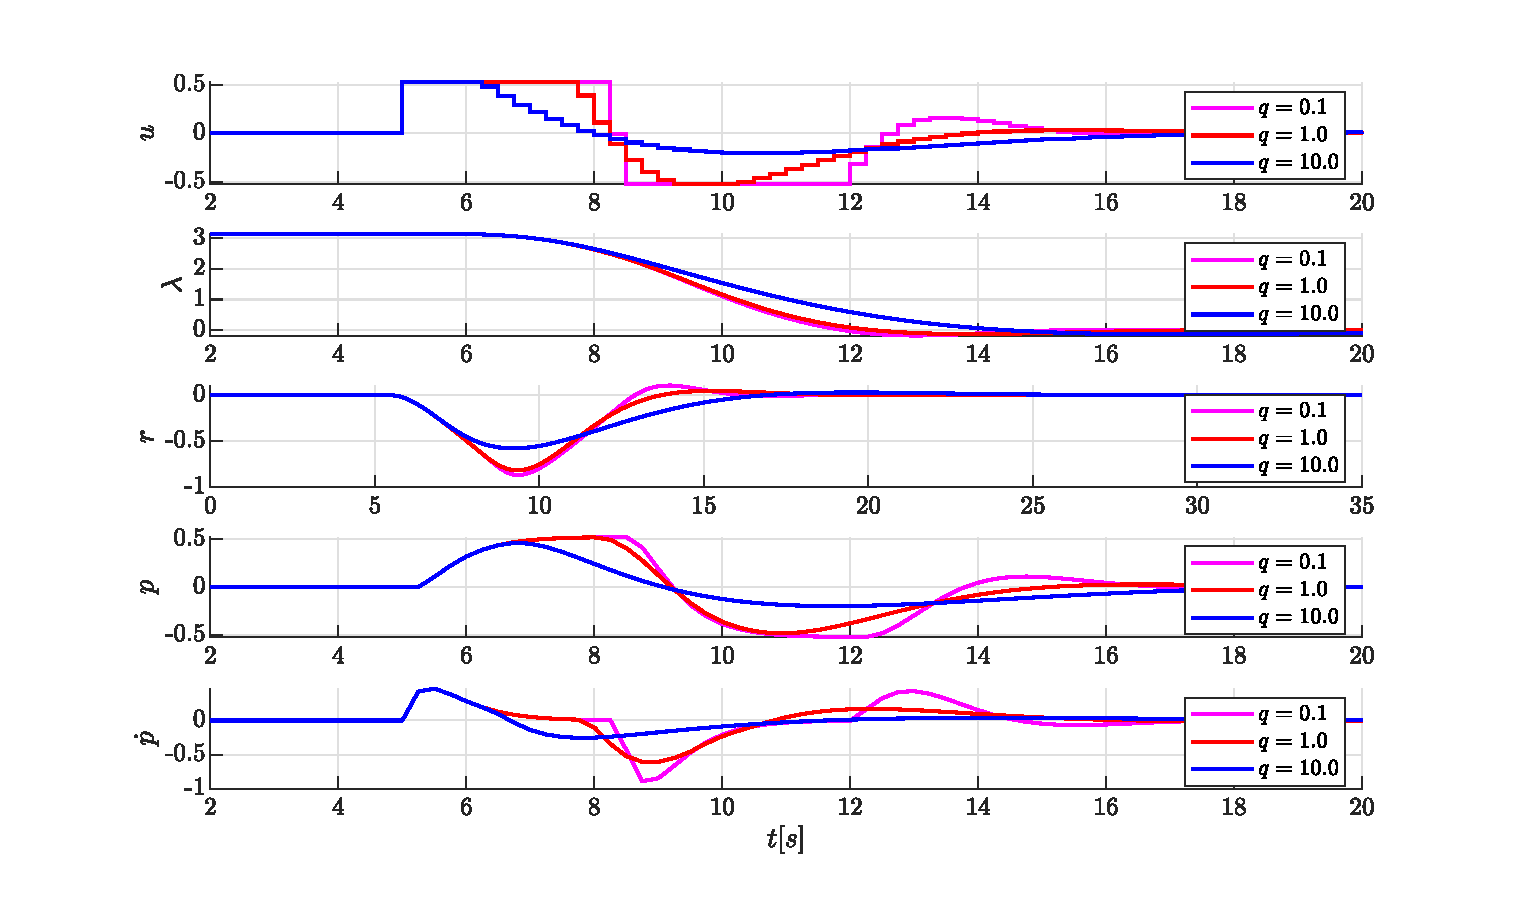
\includegraphics[width=\linewidth]{figures/lab2_optimal_u}
	\caption{Optimal trajectories for the manipulated variable and outputs with different values of $q$.}
	\label{fig:lab2_optimalu}
\end{figure}

\Cref{fig:lab2_optimalu} also shows how the constraints work in practice. Studying the plot of $ u $, we can see that no matter how low $ q $ is, the input never goes beyond the specified range of $ \pm\frac{30}{180} \pi $.

\subsection{The objective function}
\textit{Furthermore, discuss the objective function (15) (in the lab assignment text) in particular the term $(\lambda_i-\lambda_f )^2$. For instance, could any unwanted effects arise from steering the helicopter to $\lambda =\lambda_f$ with this objective function?}

The term $(\lambda_i-\lambda_f )^2$ in \cref{eq:lab2_start_cost_func} may cause problems if it becomes too large compared to the term $ q \cdot u^2 $. What is meant by ``too large'' is that the solution will actually never reach $ \lambda_f $ in the given time horizon, because it is theoretically impossible due to the problem constraints. \Cref{fig:lab2_too_large} shows this. This is the solution of the optimization problem when the group used $ \lambda_0 = 40\pi $. It shows that when the error term for the travel is too large, the helicopter will never reach $ \lambda_f $ no matter what. A direct consequence of this is that the helicopter will never stop the rotation before the time horizon ends.
\begin{figure}[h]
	\centering
	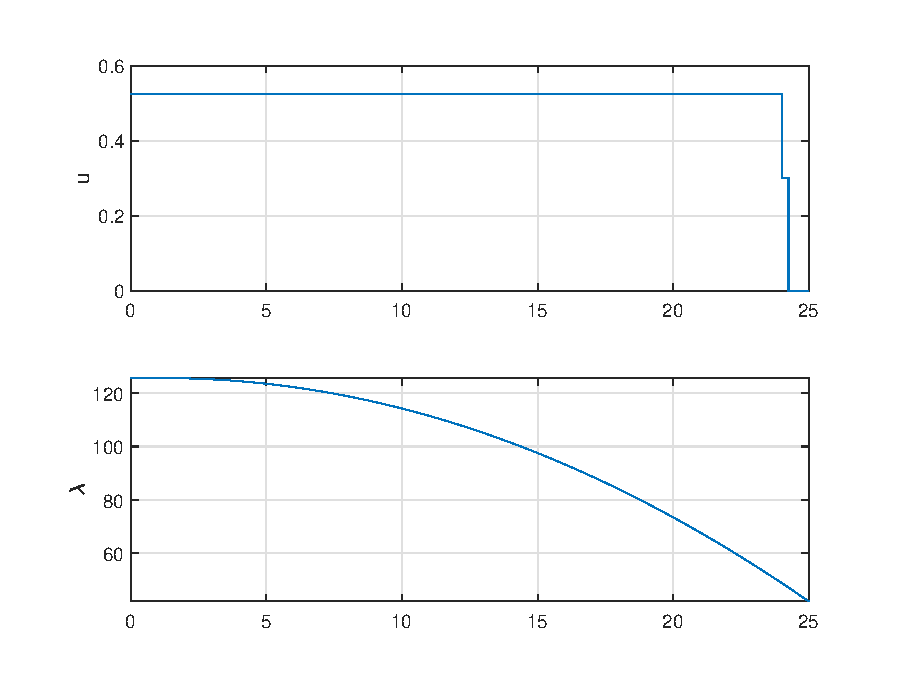
\includegraphics[width=\linewidth]{figures/lab2_1_5_example.eps}
	\caption{Optimal trajectories using $\lambda_0 = 40\pi$ .}
	\label{fig:lab2_too_large}
\end{figure}
\Cref{fig:lab2_too_large} also shows that increasing $(\lambda_i-\lambda_f )^2$ has the same effect as increasing $ \bm Q $ relative to $ r $ in \cref{eq:lab2_LQR}; it will prioritize to minimize $(\lambda_i-\lambda_f )^2$ and use much input to achieve this. We say that the ``fuel'' is cheap.

The ``solution'' to this problem is to increase the time horizon either by adding more steps (increase $N$) or increase the sampling time. This will give the optimization problem enough time to reach the $ \lambda_f $. This is shown in \cref{fig:lab2_inc_delta_t}. In this case the sampling time was doubled from $ 0.25 $ to $ 0.5 $, and the optimization problem had almost enough time to stop rotating at the final value. 
\begin{figure}[h]
	\centering
	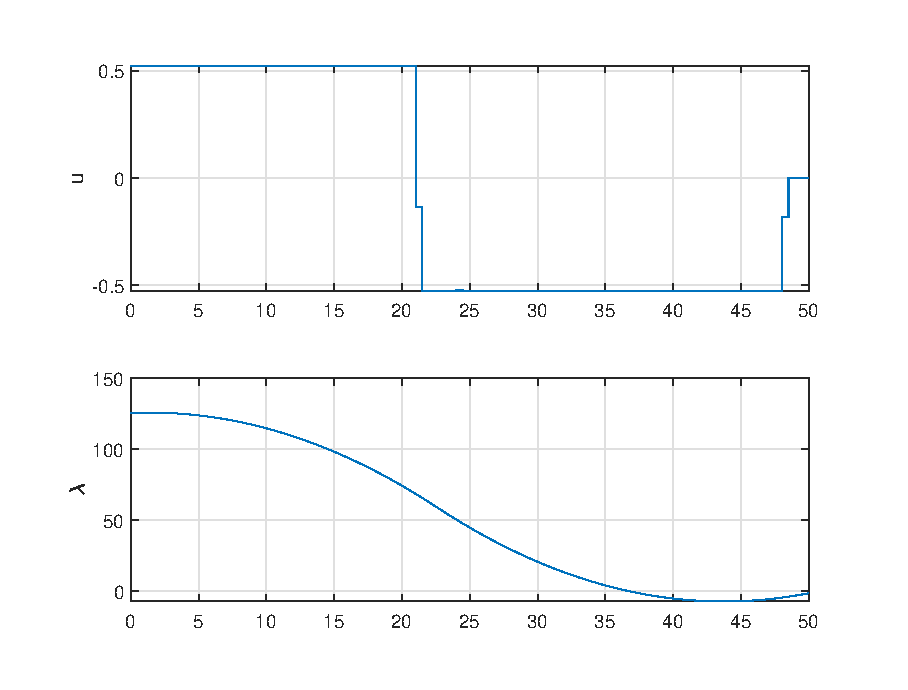
\includegraphics[width=\linewidth]{figures/lab2_1_5_example_2.eps}
	\caption{Optimal trajectories using $\lambda_0 = 40\pi$ and $ \Delta t = 0.5$ .}
	\label{fig:lab2_inc_delta_t}
\end{figure}

\subsubsection{Improved $ \lambda_0 $ selection}
In the case of the lab setup, it does not really make any sense to have $ \lambda_i-\lambda_f >  2\pi $, because the helicopter is always on a circles edge. The result of this is that $ \lambda = 0 $, $ \lambda = 2\pi $ and $ \lambda = 4\pi $ and so on, is essentially the same helicopter-configuration. 

Also, the way the objective function is set up, it will not choose the always choose the shortest way to $ \lambda_f $. If $ \lambda_0 = \frac{3}{4} \pi $, this means that the helicopter is $\frac{3}{4} \pi $ radians from $ \lambda_f $ in the counter-clockwise direction and  $\frac{1}{4} \pi $ radians from  $ \lambda_f $ in the clockwise direction. Therefore, it is most logical to go the clockwise direction, because this requires the least amount of input. However, the way the objective function is chosen, it will go in the counter-clockwise direction.

Therefore, a suggested solution from the group, is to use the following formula for $ \lambda_0 $: 
\begin{subequations}
	\begin{align}
		\lambda_{0, \text{modified}} &= \begin{cases}
			+\text{mod}(\lambda_0-\lambda_f, 2\pi), \quad &\text{if} \quad \text{mod}(\lambda_0-\lambda_f, 2\pi) \leq \pi \\
			-(2 \pi - \text{mod}(\lambda_0-\lambda_f, 2\pi)) \quad &\text{else}
		\end{cases} \\ 
	\end{align}
\end{subequations}, where $ \text{mod} $ is the modulus operator.

This will insure that $ \lambda_i-\lambda_f \leq  2\pi $ for all $ i \in (0, 1, 2, ..., N-1) $ and it will also insure that the helicopter will choose the shortest direction.

It is easily implemented in the code, as \cref{lst:improved_lambda_0} shows.
\begin{lstlisting} [caption={Improved $\lambda_0$ implementation.}, label={lst:improved_lambda_0}]
	lambda_0 = 4/3*pi; %Some value
	lambda_0 = mod(lambda_0, 2*pi);
	if (lambda_0 > pi)
		lambda_0 = -(2*pi - lambda_0);
	end
\end{lstlisting} 

\clearpage
\subsection{Experimental results}\label{kap:task_10_2_experimental_results}
The group performed two experiments with the helicopter:
\begin{enumerate}
	\item Flight with optimal setpoints: $u_k = u_k^*$
	\item Flight without setpoints: $u_k = 0$
\end{enumerate}
Both fligths, along with the optimal trajectory and a compensated trajectory are plotted in \cref{fig:LAB2_plot_1}.

\begin{figure}[h]
	\centering
	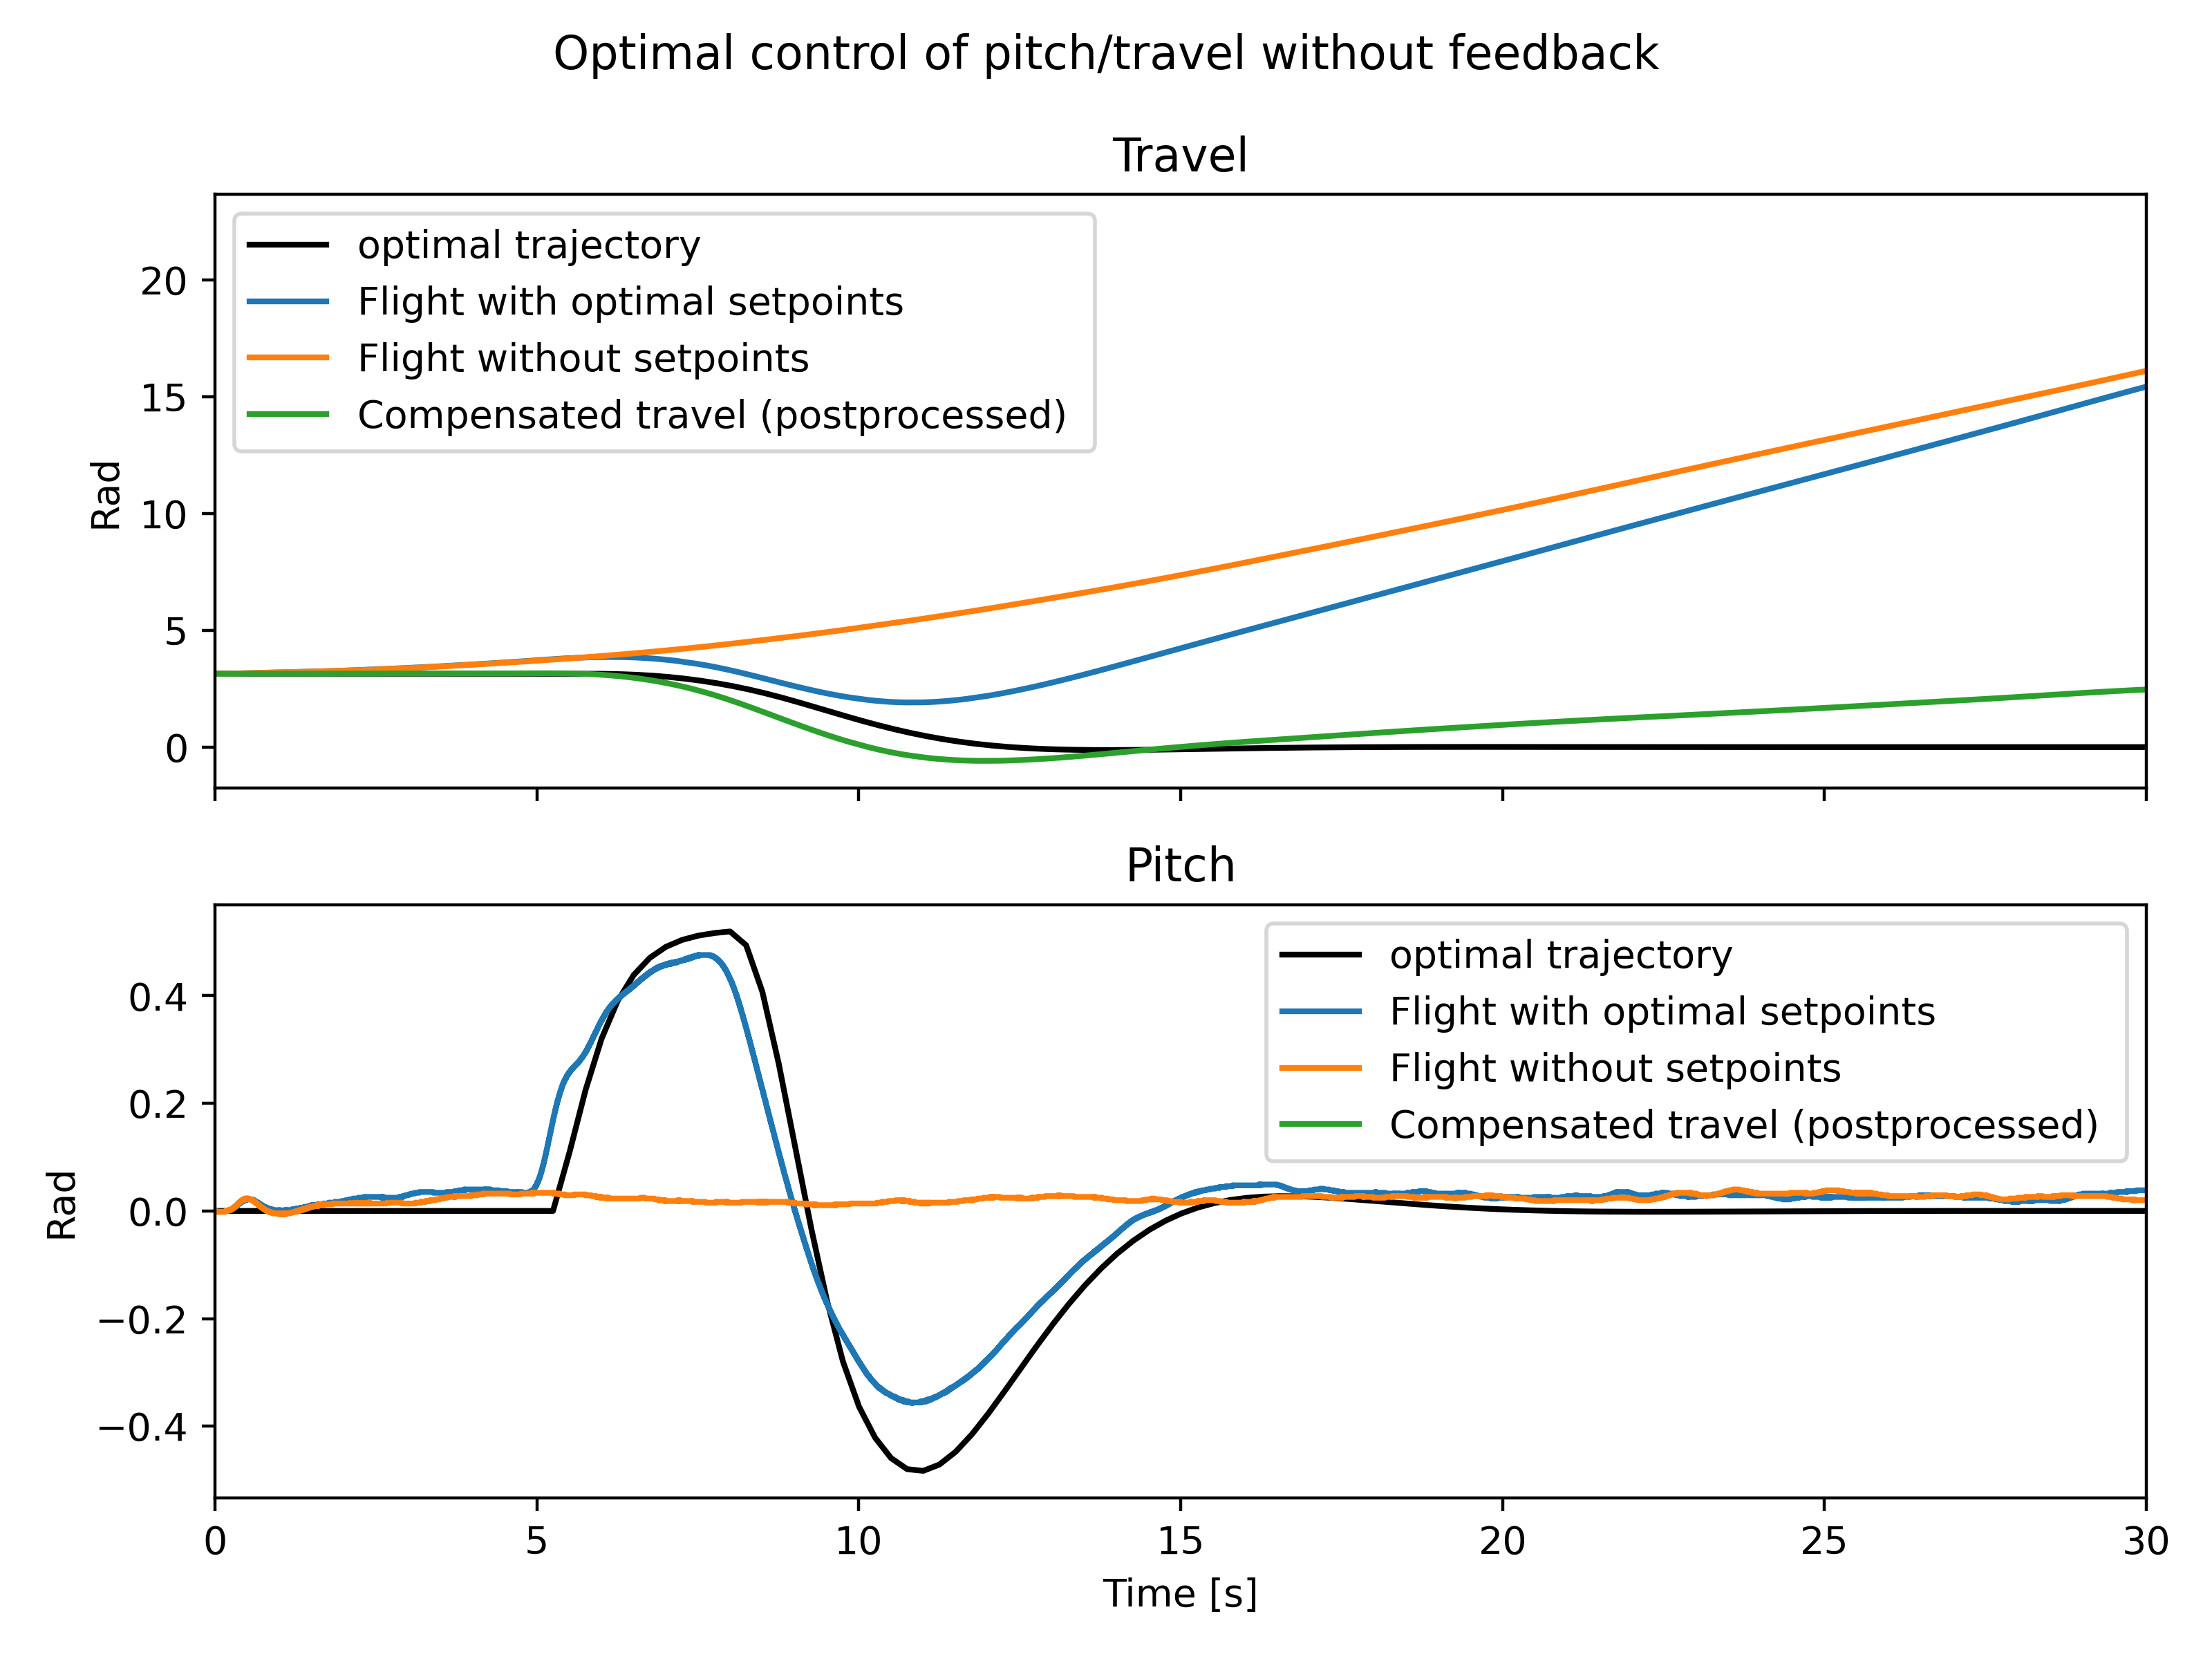
\includegraphics[width=0.8\linewidth]{figures/LAB2_plot_1.png}
	\caption{Results of LAB2}
	\label{fig:LAB2_plot_1}
\end{figure}

\subsubsection{Pitch-control}
It is clear that both fligths have adequate control of pitch. In the case where $u_k = 0$ the pitch is close to $0$. In the case where $u_k = u_k^*$ the pitch is close to the optimal trajectory.

This is expected as pitch-control is a closed loop - the basic control layer has a PD controller that ensures that pitch follows the reference $u_k$.

\subsubsection{Travel-drift}\label{kap:LAB2_travel_drift_causes}
From the flight with $u_k = 0$ it is clear that there is significant travel-drift present in the helicopter. Even when pitch is very close to $0$ the helicopter travels quickly far away from the initial point.

There are three main causes of drift:
\begin{enumerate}
	\item The encoder-measurement of pitch is not precise
	\item Helicopter inbalance
	\item Disturbances
\end{enumerate}

When the helicopter starts, it reads the initial \textbf{encoder}-value for the pitch, and assumes this is equal to zero. However, if the platform is not built precisely, the encoder axis may not be 100 \% aligned with the corresponding real world axis. There are many possible reasons for this, but it will not be discussed further. Regardless of the cause, the effect will be the same: The measured encoder-value will have a constant offset compared to real world-values. This will again cause the helicopter to drift when it measures zero pitch.

%The \textbf{encoder} does not measure pitch at the helicopter in relation to gravity, rather it measures the angle between the helicopter blades and the platform that holds them. Because that platform is not build to be precisely the same as gravity (and because of wear-and-tear) the measured value $0$ is not exactly 0. This causes the helicopter to have a pitch offset, which in turn generates travelrate and travel.

The \textbf{imbalance} may be that one rotor is stronger than the other, or that the rotors have offsets from the vertical position. These imbalances may generate a sidewards force, even when the helicopter is pitched to $0$, which in turn generates travelrate and travel.

The \textbf{disturbances} is the most general effect. Air-pressure, wind, temperature effects, walls, and so on. All of these disturbances may cause drifts or noise in the travel. 

The group believes that the main cause of the drift observed in the helicopter is the offset in the encoder.

\subsubsection{Conclusion}
As \cref{fig:LAB2_plot_1} clearly shows the control sequence did not yield the desired travel-response. This was expected, as there are many causes of drift and disturbances. Without any feedback the helicopter will quickly deviate from the desired response, since it will not have any mechanisms to detect deviations from the optimal trajectories.

Nevertheless it is possible to verify the control sequence by compensating for the drift. The compensation can be done by taking the travel of the flight with optimal setpoints, and subtracting the drift logged in the flight without setpoints (i.e. $ u_k = 0 $). The result is plotted as compensated travel in \cref{fig:LAB2_plot_1}. This clearly shows that without the major drift the helicopter would be much closer to the optimal trajectory.


\clearpage
\subsection{MATLAB and Simulink}
\subsubsection{MATLAB}
\lstinputlisting[caption= {MATALB code for lab 2}, label={lst:lab2_matlab}]{code/lab2.m}
\clearpage
\subsubsection{Simulink}
\begin{figure}[h]
	\centering
	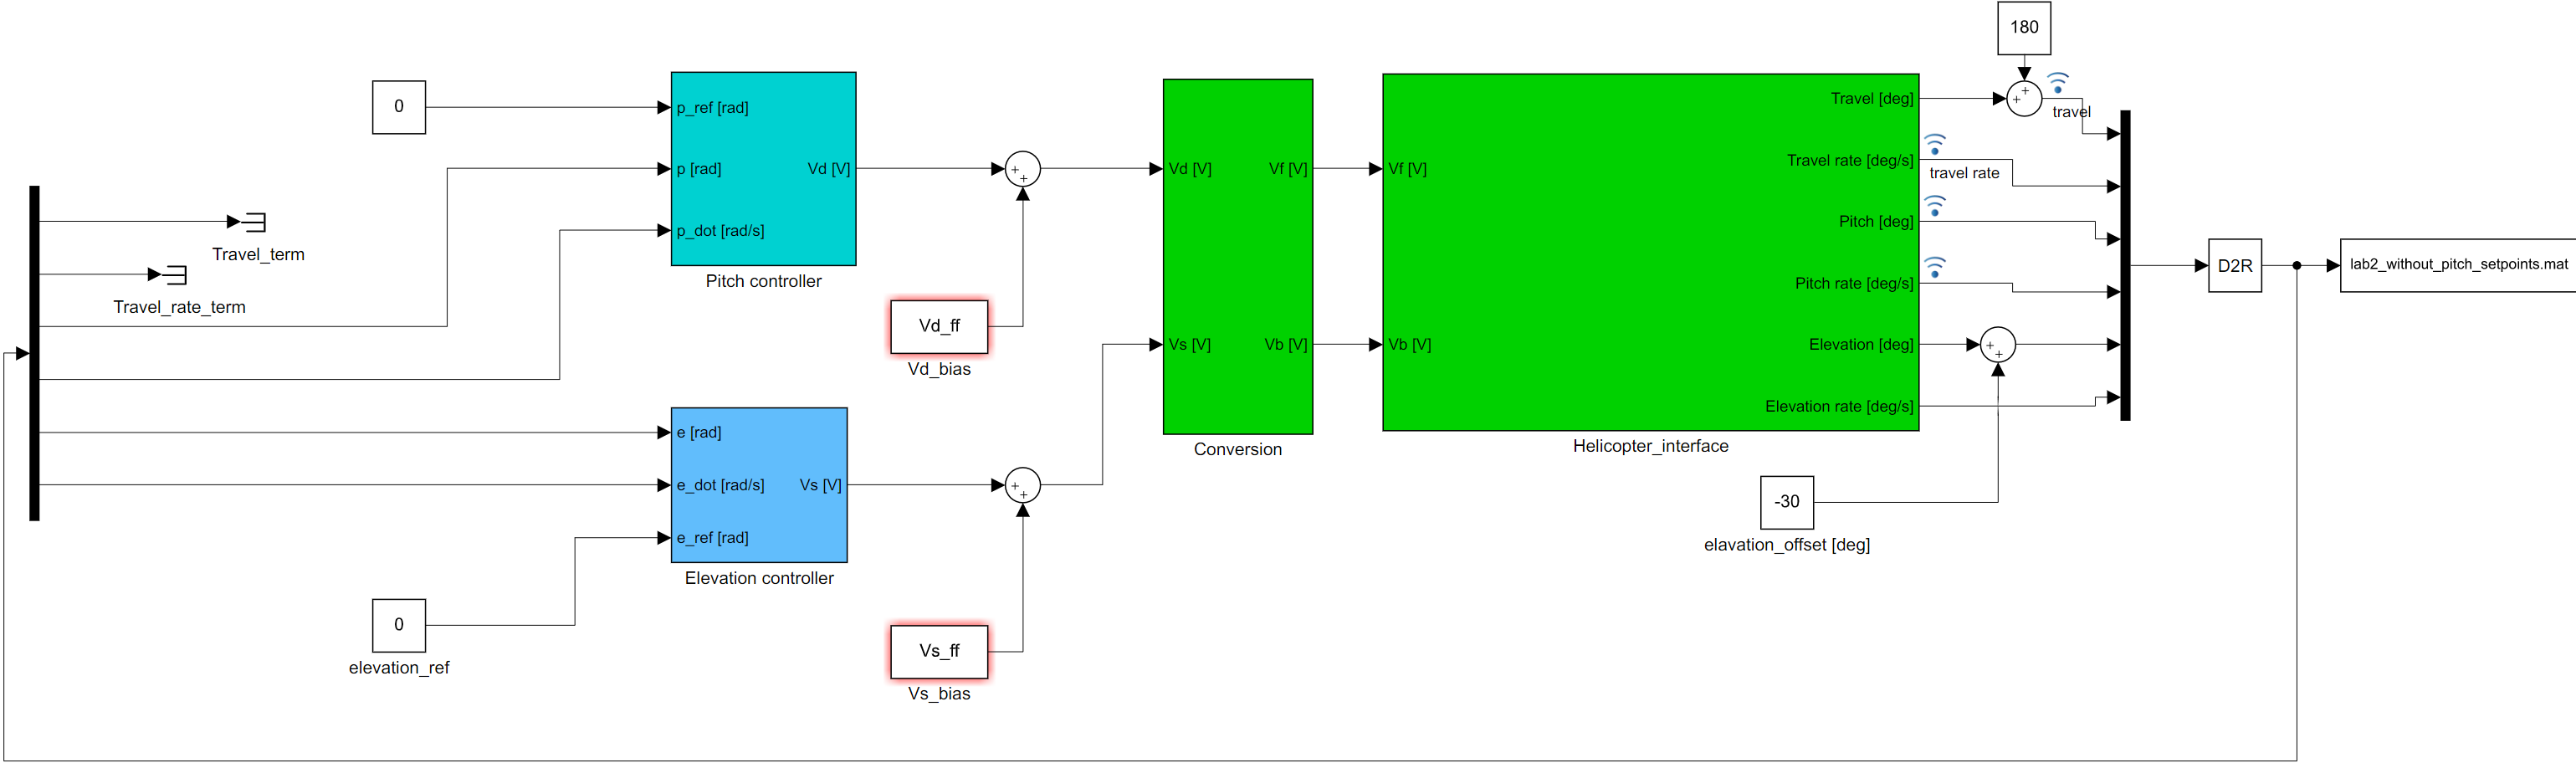
\includegraphics[angle=90, width=0.5\textwidth,height=0.7\textheight]{code/lab2_simulink}
	\caption{Simulink diagram used in lab 2.}
	\label{fig:lab2_simulink}
\end{figure}
\end{document}
\documentclass[../main.tex]{subfiles}
\begin{document}

\section{Optimal Control of Pitch/Travel with Feedback (LQ)}  \label{sec:lab3}
In this task we add feedback to the optimal controller that we developed in \cref{kap:Part2OptimalControlWithoutFeedback}.

\subsection{Motivation}
The experimental results in \cref{kap:task_10_2_experimental_results} clearly shows that planning a sequence of inputs does not produce the expected sequence of outputs - as that section explains there are many reasons for travel-drift. In situations with drift without feedback then the output will not follow the planned trajectory, but adding feedback could compensate for the drift and offset and therefore reduce or eliminate the deviation from the planned trajectory.

The results achieved in this section shows that adding feedback greatly improves performance.

\subsection{Introducing feedback}
There are many approaches to adding feedback, but in this assignment only two will be considered: linear state feedback and model predictive control.

\textbf{Linear state feedback} adds a new control layer below the optimization layer, the advanced control layer, that controls the setpoint to the pitch controller. The setpoint is determined from a control law that considers the optimal trajectory and the current state of the system. If the states deviate from the optimal value the input is changed according to the pitch-control equation:
\begin{equation}\label{eq:lab3_feedback}
	u_k = u_k^* - \bm{K}^T(\bm x_k - \bm x_k^*)
\end{equation}
where $u_k^*$ and $\bm x_k^*$ are the optimal input and state trajectories predicted in the optimization layer, $u_k$ is the next input and $x_k$ is the current state. $K$ is the linear state feedback gain. 

In this exercise the gain matrix $K$ is calculated as an infinite horizon LQ controller, see \cref{kap:task_10_3_LQ_controller} for more info about the exact implementation.

\textbf{Model Predictive Control (MPC)} is a completely different solution: the optimal trajectory is recalculated at every timestep - instead of compensating for deviation from optimal, the optimal is recalculated to get a new possible trajectory based on the current states. See \cref{kap:10_3_mpc} for more info about how that could be implemented here.

\subsection{LQ controller} \label{kap:task_10_3_LQ_controller}
A Linear Quadratic (LQ) controller minimizes the quadratic objective function:
\begin{equation}
    J = \sum^\infty_{i=0} \Delta x_{i+1}^\top Q \Delta x_{i+1} + \Delta u_i^\top R \Delta u_i, \quad Q \ge0, \quad R > 0
\end{equation}
for a linear model
\begin{equation}\label{eq:lab3_lin_model}
	\Delta x=A\Delta x_i + B \Delta u_i
\end{equation}
Here $ \Delta x = x - x^*$ and $\Delta u = u - u^*$ are deviations from the optimal trajectory.

This formulation is an infinite horizon linear quadratic regulator which has a solution with a constant linear feedback gain, $K$ - which is exactly what was specified previously! Note that this regulator does not have any constraints.

\subsubsection{Choosing the weights} 
The matrix $Q$ and the scalar $R$ are the weights of the optimalization problem. $Q$ determines how much state-deviations should be penalized, while $R$ determines how much input-deviation should be penalized. What needs to prioritized depends on the application.

In this case the system is a helicopter where the goal is to control the travel of the helicopter. The travel is the most important state, while travelrate, pitch and pitchrate are secondary. Thus it makes sense to prioritize keeping travel close to the planned trajectory - it is of course not possible to keep all states close to the trajectory. This motivates a \textbf{state-weight} with relatively high value related to travel.

The LQR regulator controls the pitch-setpoint that in turn controls travel. In the end controlling travel is the most important - a deviation in setpoint from the predicted optimal is completely fine as this is how travel is regulated. Thus a low input-weight is warranted as that allows the setpoint to deviate further from the planned trajectory.

\subsubsection{Respecting constraints}
The pitch-setpoint in the optimalization layer has a constraint, see \cref{sec:lab2_constraints} - but the implementation of LQR controller does not respect this constraint! The result is that the pitch-setpoint could fall outside the constraint imposed in the optimalization layer. This does in fact happen, for instance in \cref{fig:LAB3_Q_variations_travel}, where the setpoint is outside the constraint ($\approx 0.52 rad $).

The simplest solution to this problem is to respect the constraint by saturating the output of the regulator to that value. However that does makes impossble for the LQ regulator to compensate in cases where the input is already constrained, therefore it would make sense to set the saturation limit slightly higher than the constraint value to allow the regulator to work in such cases (or equivalently set the constraint lower than the saturation point).

\subsubsection{Calculating the solution}
Calculating the solution to the LQR problem is trivial using Matlab:
\begin{lstlisting}[language=Matlab]
% The discrete system described as a state space system, Ad and Bd must be defined

% W1 is the weigth of travel
% W2 is the weight of travelrate
% W3 is the weight of pitch
% W4 is the weight of pitchrate
Q = diag([W1, W2, W3, W4]);

% W5 is the weight of the input
R = W5;

% The function dlqr is used to solve the LQR problem
[K, S, e] = dlqr(Ad, Bd, Q, R);
\end{lstlisting}

\subsection{Model Predictive Control}\label{kap:10_3_mpc}
Model Predictive Control is another way of introducing feedback to an optimal control system. In an MPC controlled system the optimal response and input is recalculated at every timestep, the input used is simply the first of the optimal input values calculated at every step.

This is a drastically different approach to the LQ-method impemented in this laboratory exercise.

\subsubsection{Implementing MPC}
Implementing MPC requires a system model, cost function, current state and input control.

One could make a Matlab function that the simulink model uses at every timestep. The input to this function is the current state (either measured or estimated), while the output is connected to the pitch-regulator. The function itself has a model of the system as well as the cost function - with the state from the system the optimalization problem can be solved and the first system-input is returned to the simulink model. 

\subsubsection{Advantages of MPC}
The biggest advantage of MPC compared to the linear state feedback introduced here, is that MPC generates a new optimal trajectory that is more realistic for the helicopter to achieve. Since the optimal trajectory is recalculated based on the current state, the helicopter's response will achieve smaller errors compared to the optimal trajectory. 

%Imagine a situation where the helicopter needs to fly below some obstacle. A deviation in elevation that would cause a collision with the obstacle might not be corrected before travel reaches the obstacle - MPC would slow down travel enough to have a trajectory that is possible to achieve.

Another advantage is that MPC allows for feedback with explicitly defined constraints. This is a more intuitive way of keeping the helicopter stable and within the wanted working-range, compared to looking at eigenvalues of the system matrix with linear state feedback.

\subsubsection{Disadvantages of MPC}
The biggest disadvantage to MPC is complexity and computation time - in a control system there are hard deadlines and if the optimalization problem has not been solved within that deadline, the system has a problem.

First of all the problem must be simple enough or optimized enough to solve at every timestep. If this is not achievable the problem must be simplified/optimized or the timestep must be increased. The time to solve a problem can also vary, which makes this issue more complex.

Another issue is \textbf{existence of solutions} must be guaranteed for all situations. It is possible to have problems that have solutions in some configurations, while being undefined for others. Our helicopter is far from perfect, and our model is quite simple. These imperfections may cause the helicopter's configuration to go outside the defined constraints. This could cause the helicopter to freeze mid-air because there was no solution. If these border cases was not taken care of during implementation, this could be fatal.

\subsubsection{Modified Control Hierarchy with MPC}

\begin{figure}[h]
	\centering
	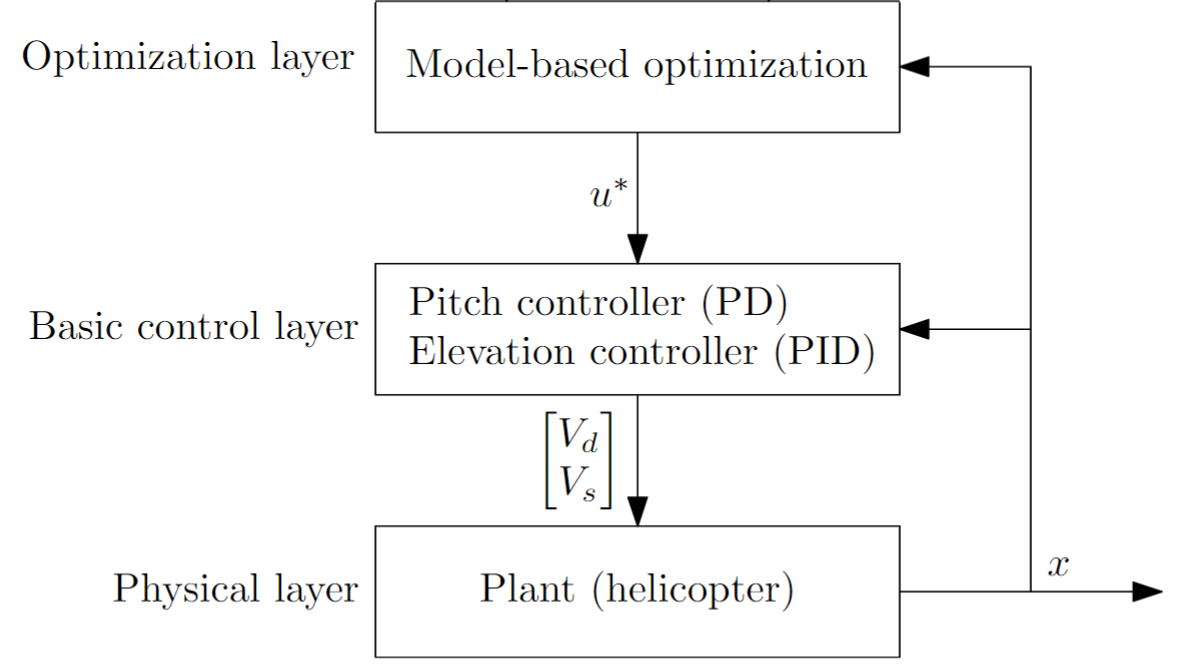
\includegraphics[width=0.7\linewidth]{content/MPC control hierarchy.png}
	\caption{The control hierarchy would look like this using MPC.}
\end{figure}

\subsection{Experimental results}\label{sec:lab3_result}
The group performed a host of controlled tests with different tunings within five different targets:
\begin{enumerate}
	\item Prioritizing input use, see \cref{fig:LAB3_R_variations}
	\item Prioritizing travel, see \cref{fig:LAB3_Q_variations_travel}
	\item Prioritizing travelrate, see \cref{fig:LAB3_Q_variations_travelrate}
	\item Prioritizing pitch, see \cref{fig:LAB3_Q_variations_pitch}
	\item Prioritizing pitchrate, see \cref{fig:LAB3_Q_variations_pitchrate}
\end{enumerate}

It is very clear that introducing feedback produced results much better than the ones achieved without feedback, almost regardless of the tuning of the LQR regulator.

Prioritizing input usage only has a slight effect, the input usage does get slightly closer to the planned trajectory but not by much. This could of course be pushed further by weighing states lower or input higher, but this was not explored - if the input is regulated very close to the planned trajectory then the result is the same as the previous lab-exercise where u was exactly equal to the planned trajectory.

Prioritizing travel has a great effect on the travel response - resulting in almost perfect travel response. Unfortunately this also introduced oscillations in pitch-setpoint, pitch and pitchrate.

Prioritizing travelrate, pitch and pitchrate results in responses closer to the corresponding planned trajectory, but this is not further discussed as travel is the state most important to control - theese experiments were only to show that it would be possble should another state be valuable.

\subsubsection{Possible improvements}
The group observed that the state never reached the optimal trajectory, even with very high Q-values. The group believes that adding integration to the LQ-regulator would eliminate the stationary offset between travel and the planned travel trajectory.

Another possible improvement would be to change the cost function in the optimalization layer to generate a trajectory that is easier for the helicopter to follow. There is not guarantee that it is physically possible for the helicopter to follow the trajectory generated here, because the model of the system is not perfect.

\subsubsection{Plots}

\begin{figure}[h]
	\centering
    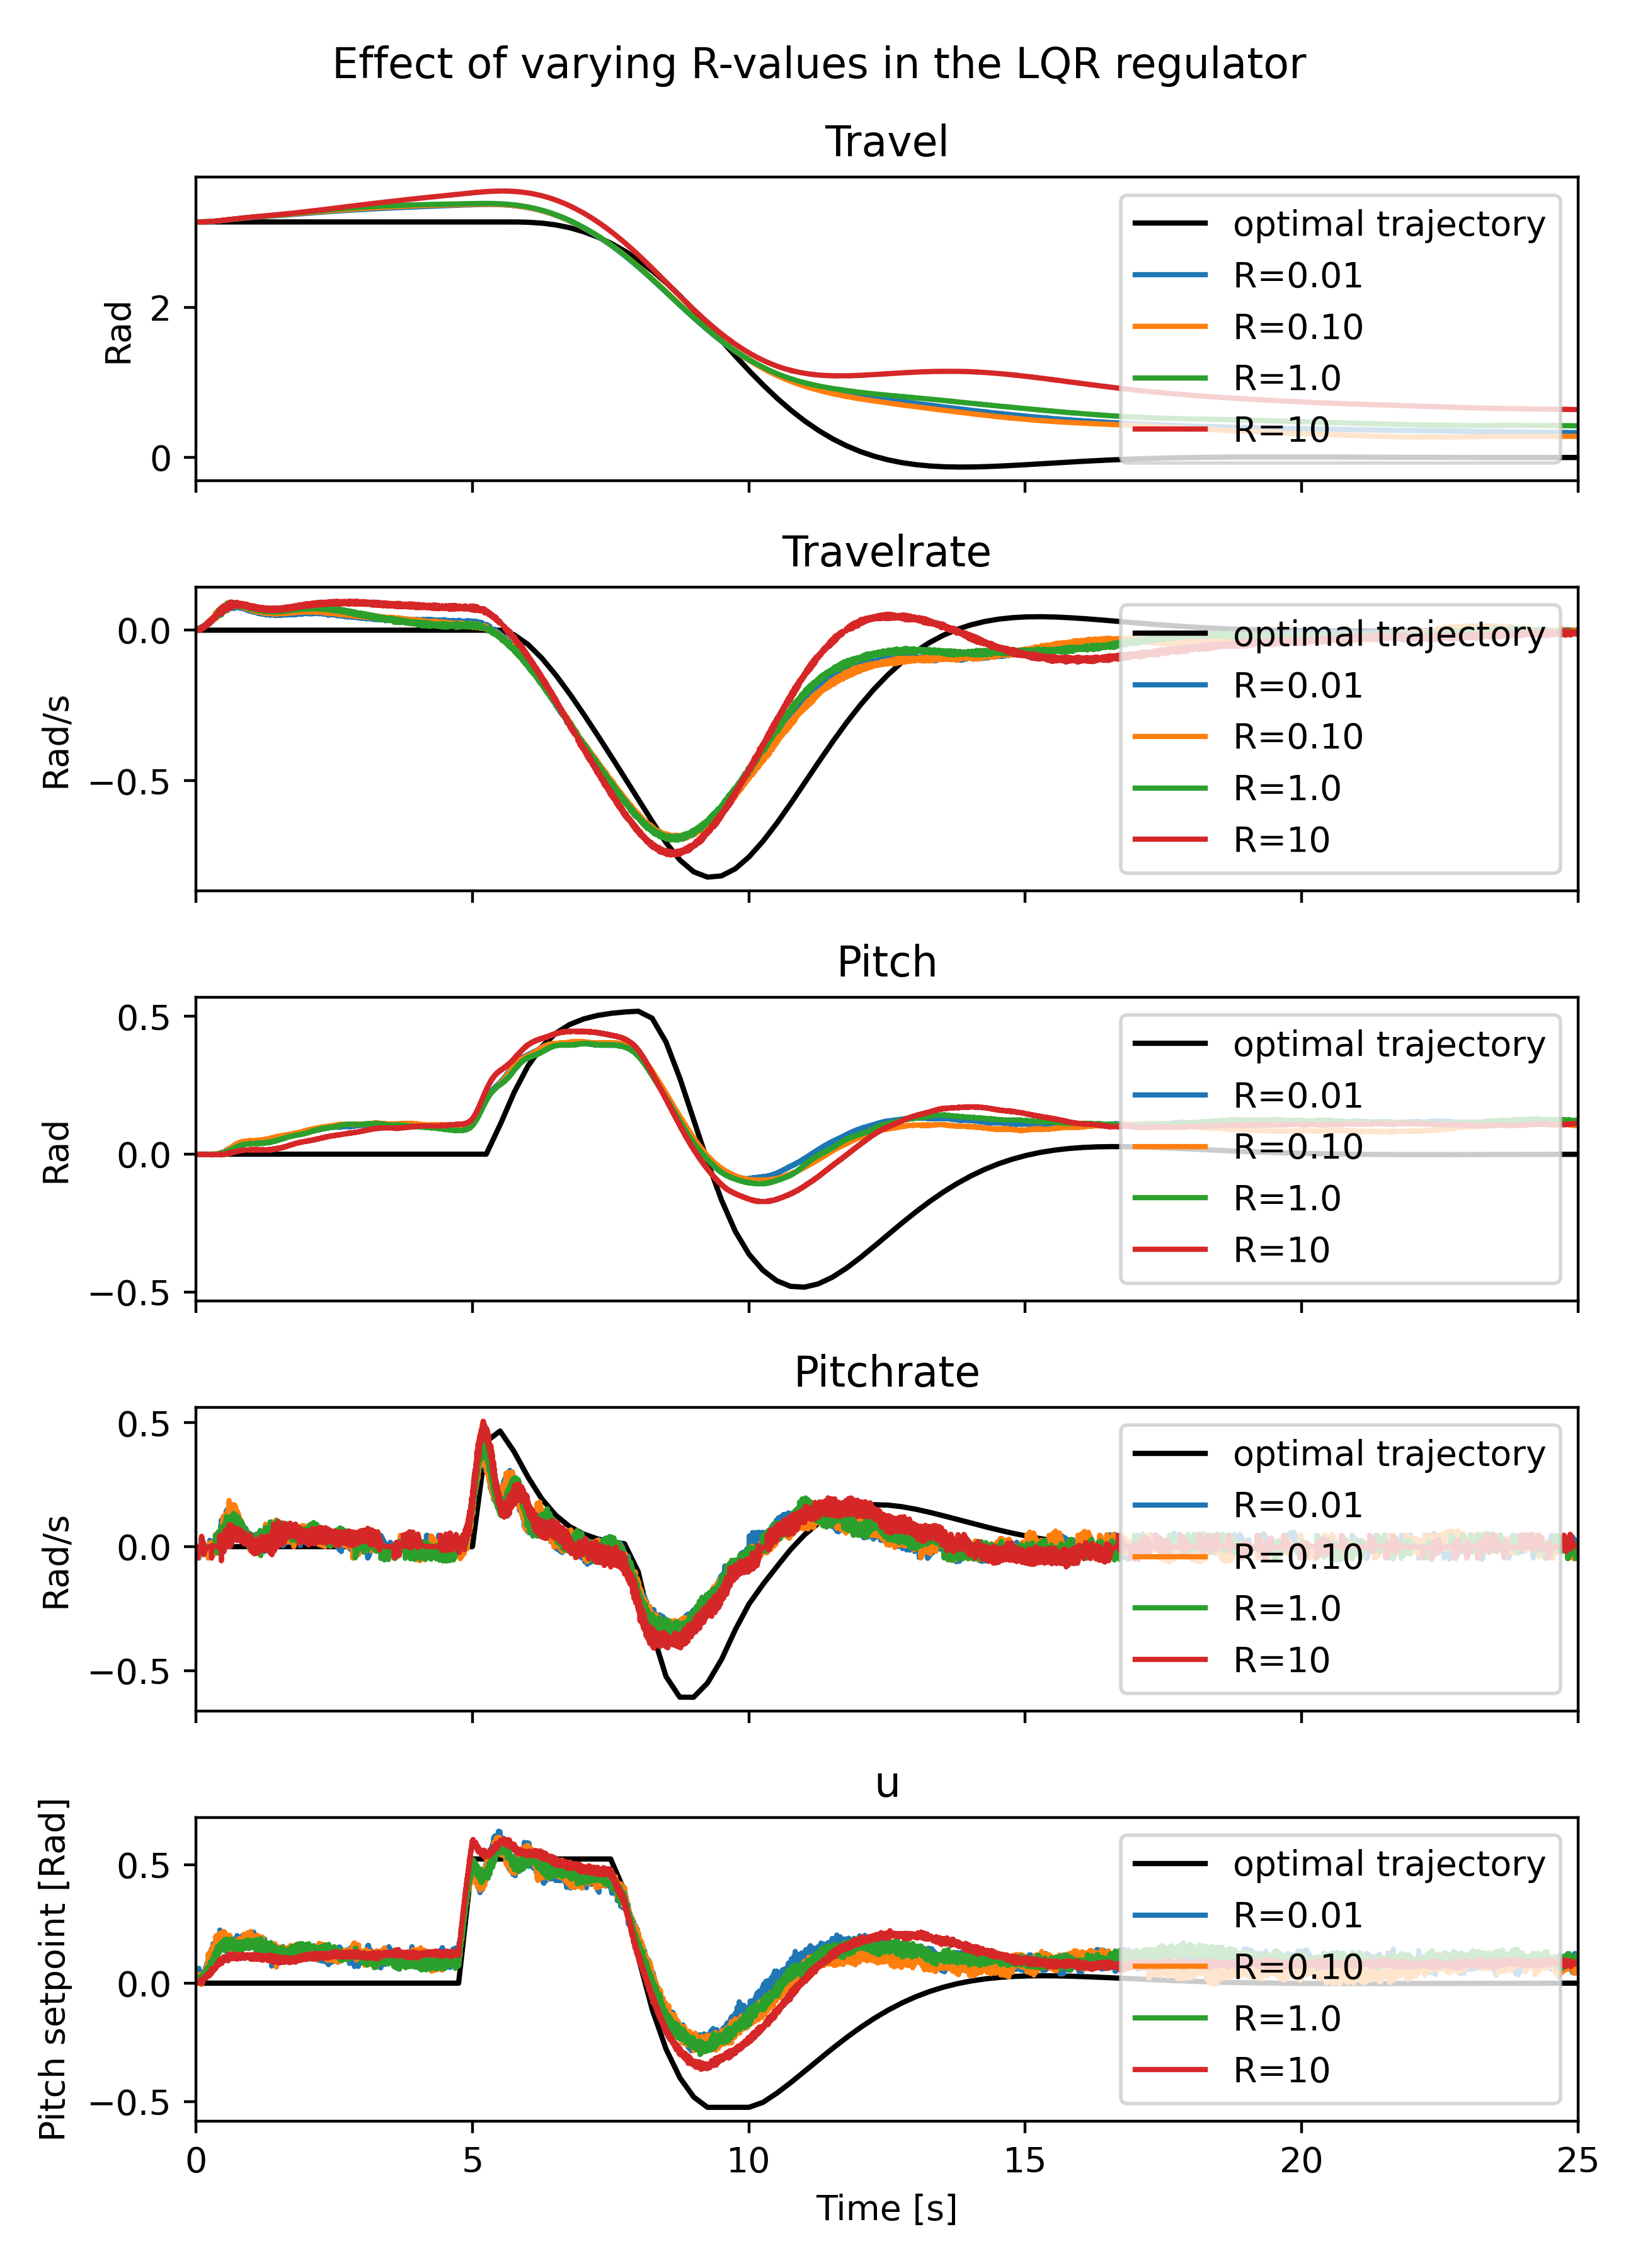
\includegraphics[width=0.8\linewidth]{figures/LAB3_R_variations.png}
	\caption{Prioritizing input-usage while keeping Q=diag([1,1,1,1]). This shows a very slight difference between weights. No further experimentation was done because if $u_k = u_k^*$ then that would be the same as the previous exercise.}
	\label{fig:LAB3_R_variations}
\end{figure}

\begin{figure}[h]
	\centering
	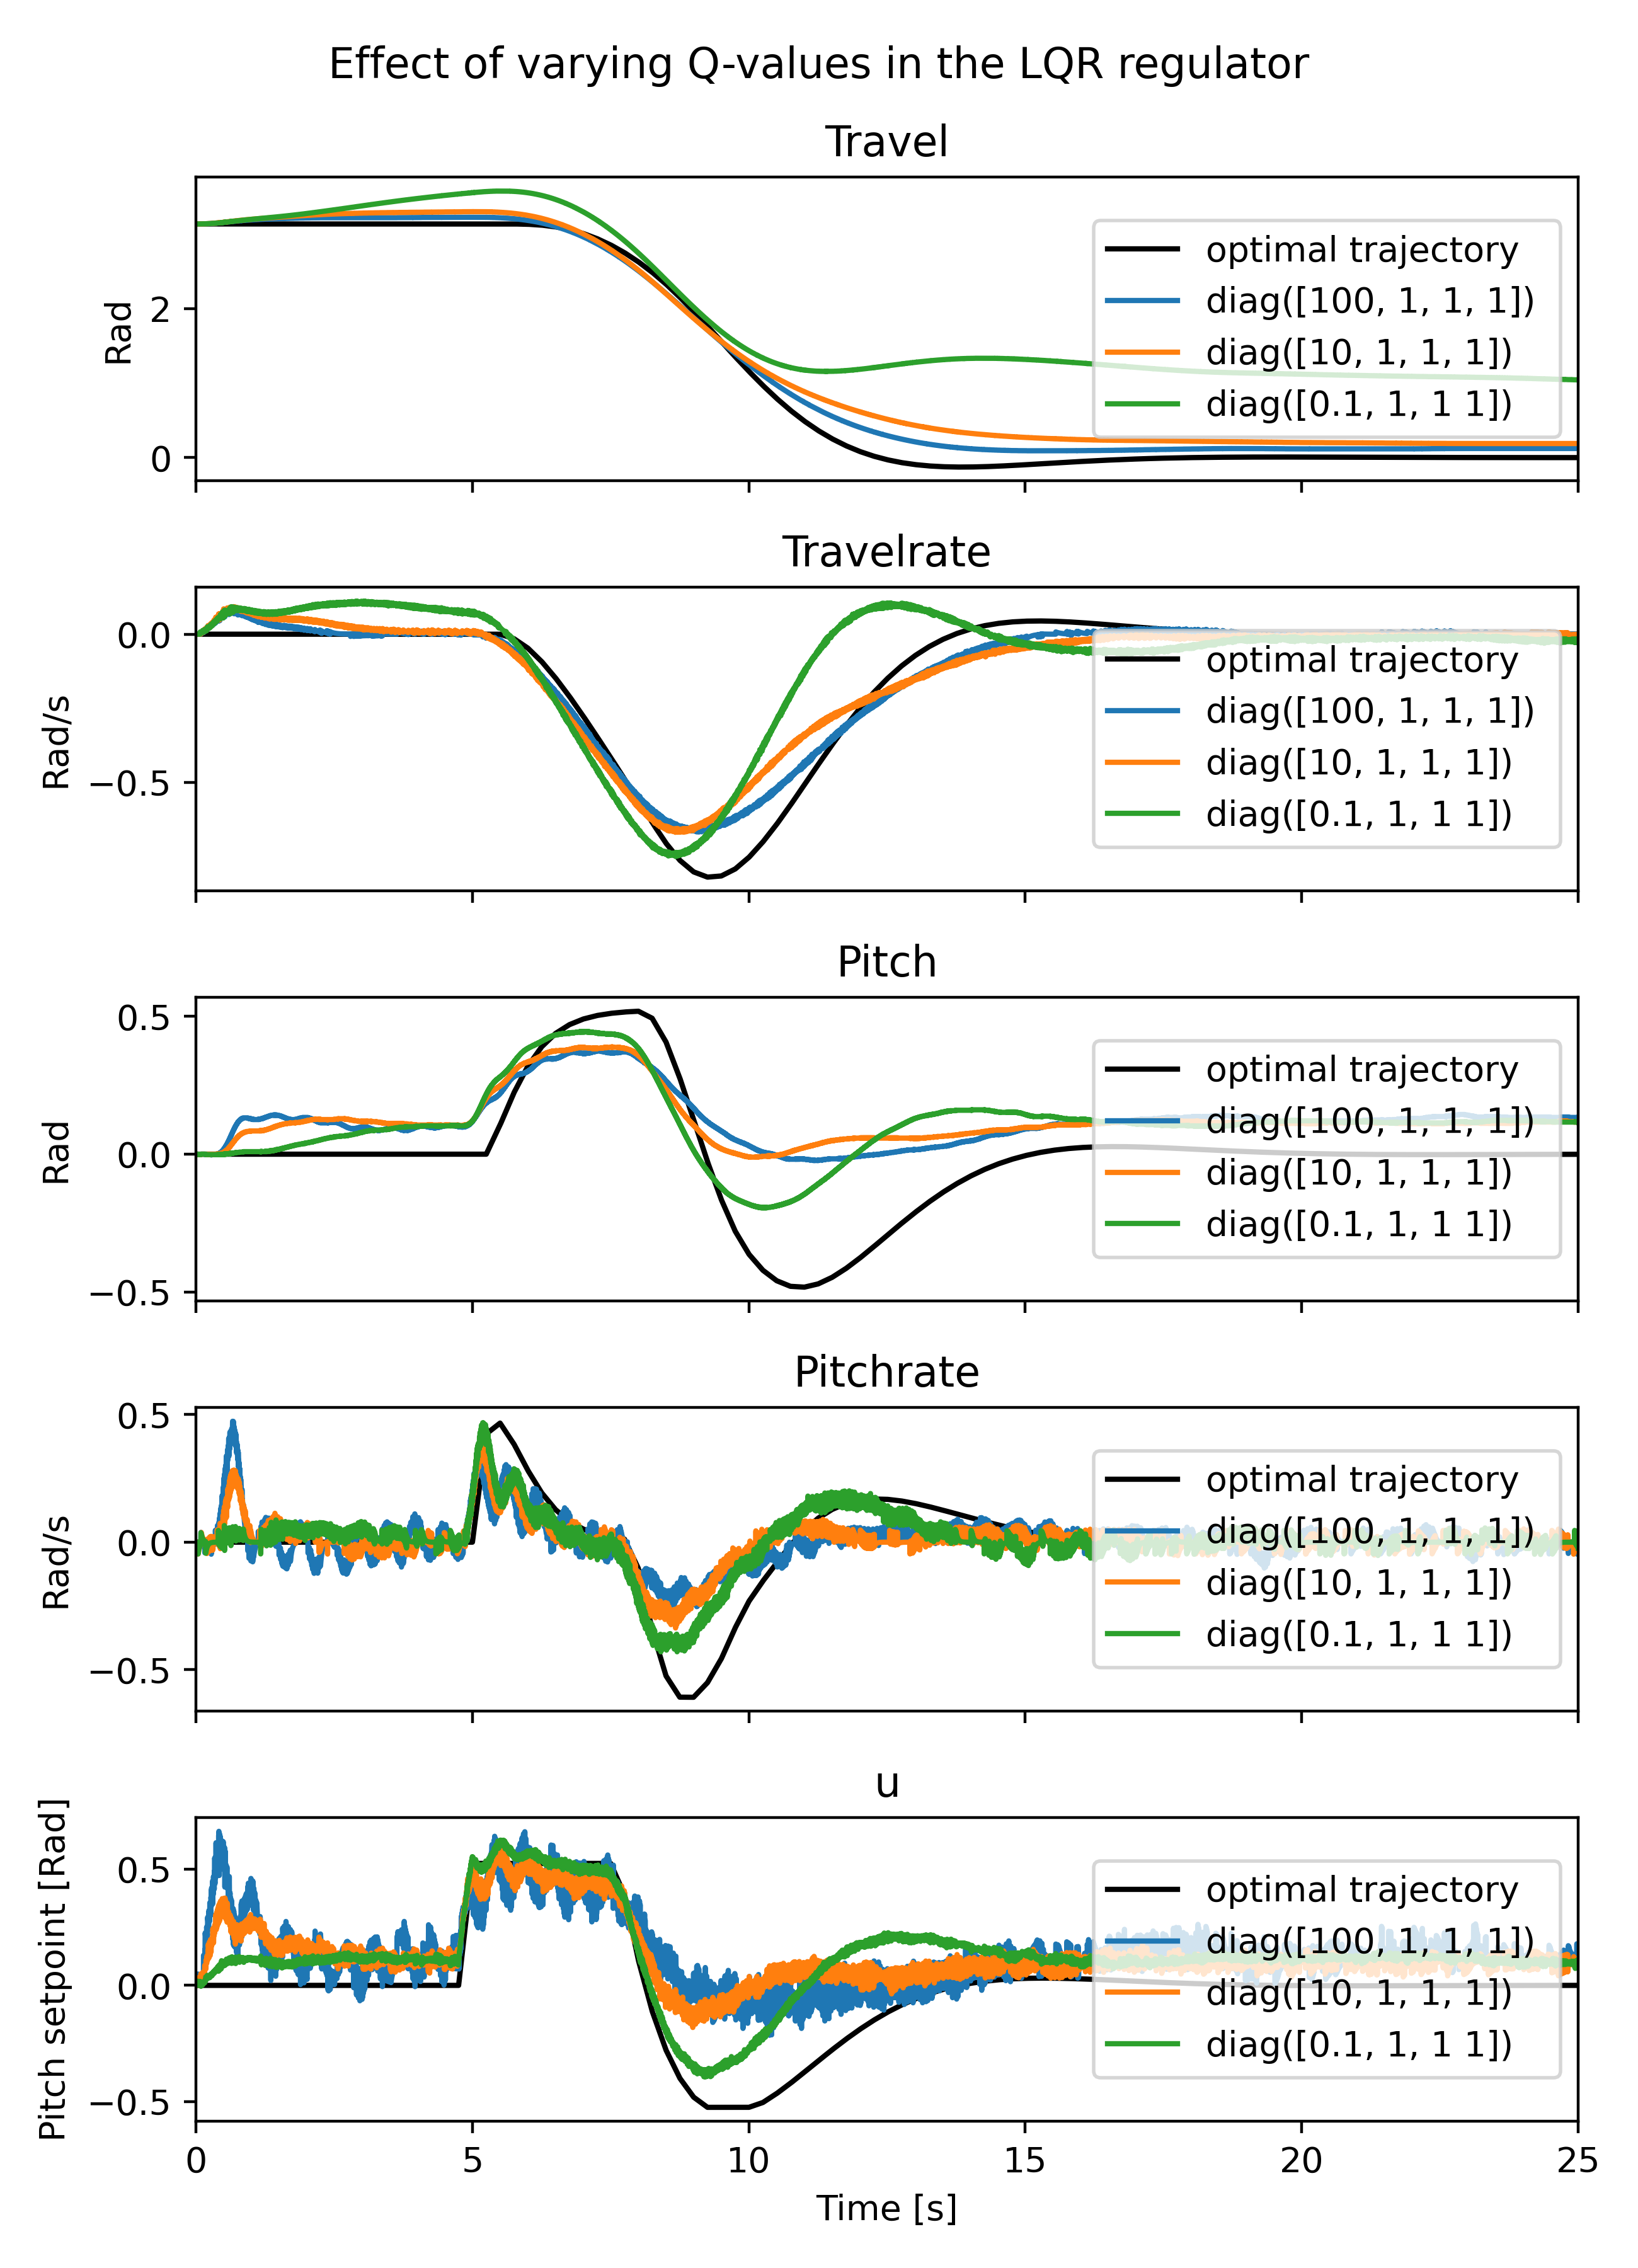
\includegraphics[width=0.8\linewidth]{figures/LAB3_Q_variations.png}
	\caption{Prioritizing the weight related to travel while keeping $R=1$. This was very effective in reducing offset between travel and the planned trajectory. Unfortunately at heigher gains there is some offset introducted and even then there is still a constant offset. A regulator with integral action would probably eliminate this offset without introducting oscillations.}
	\label{fig:LAB3_Q_variations_travel}
\end{figure}

\begin{figure}[h]
	\centering
	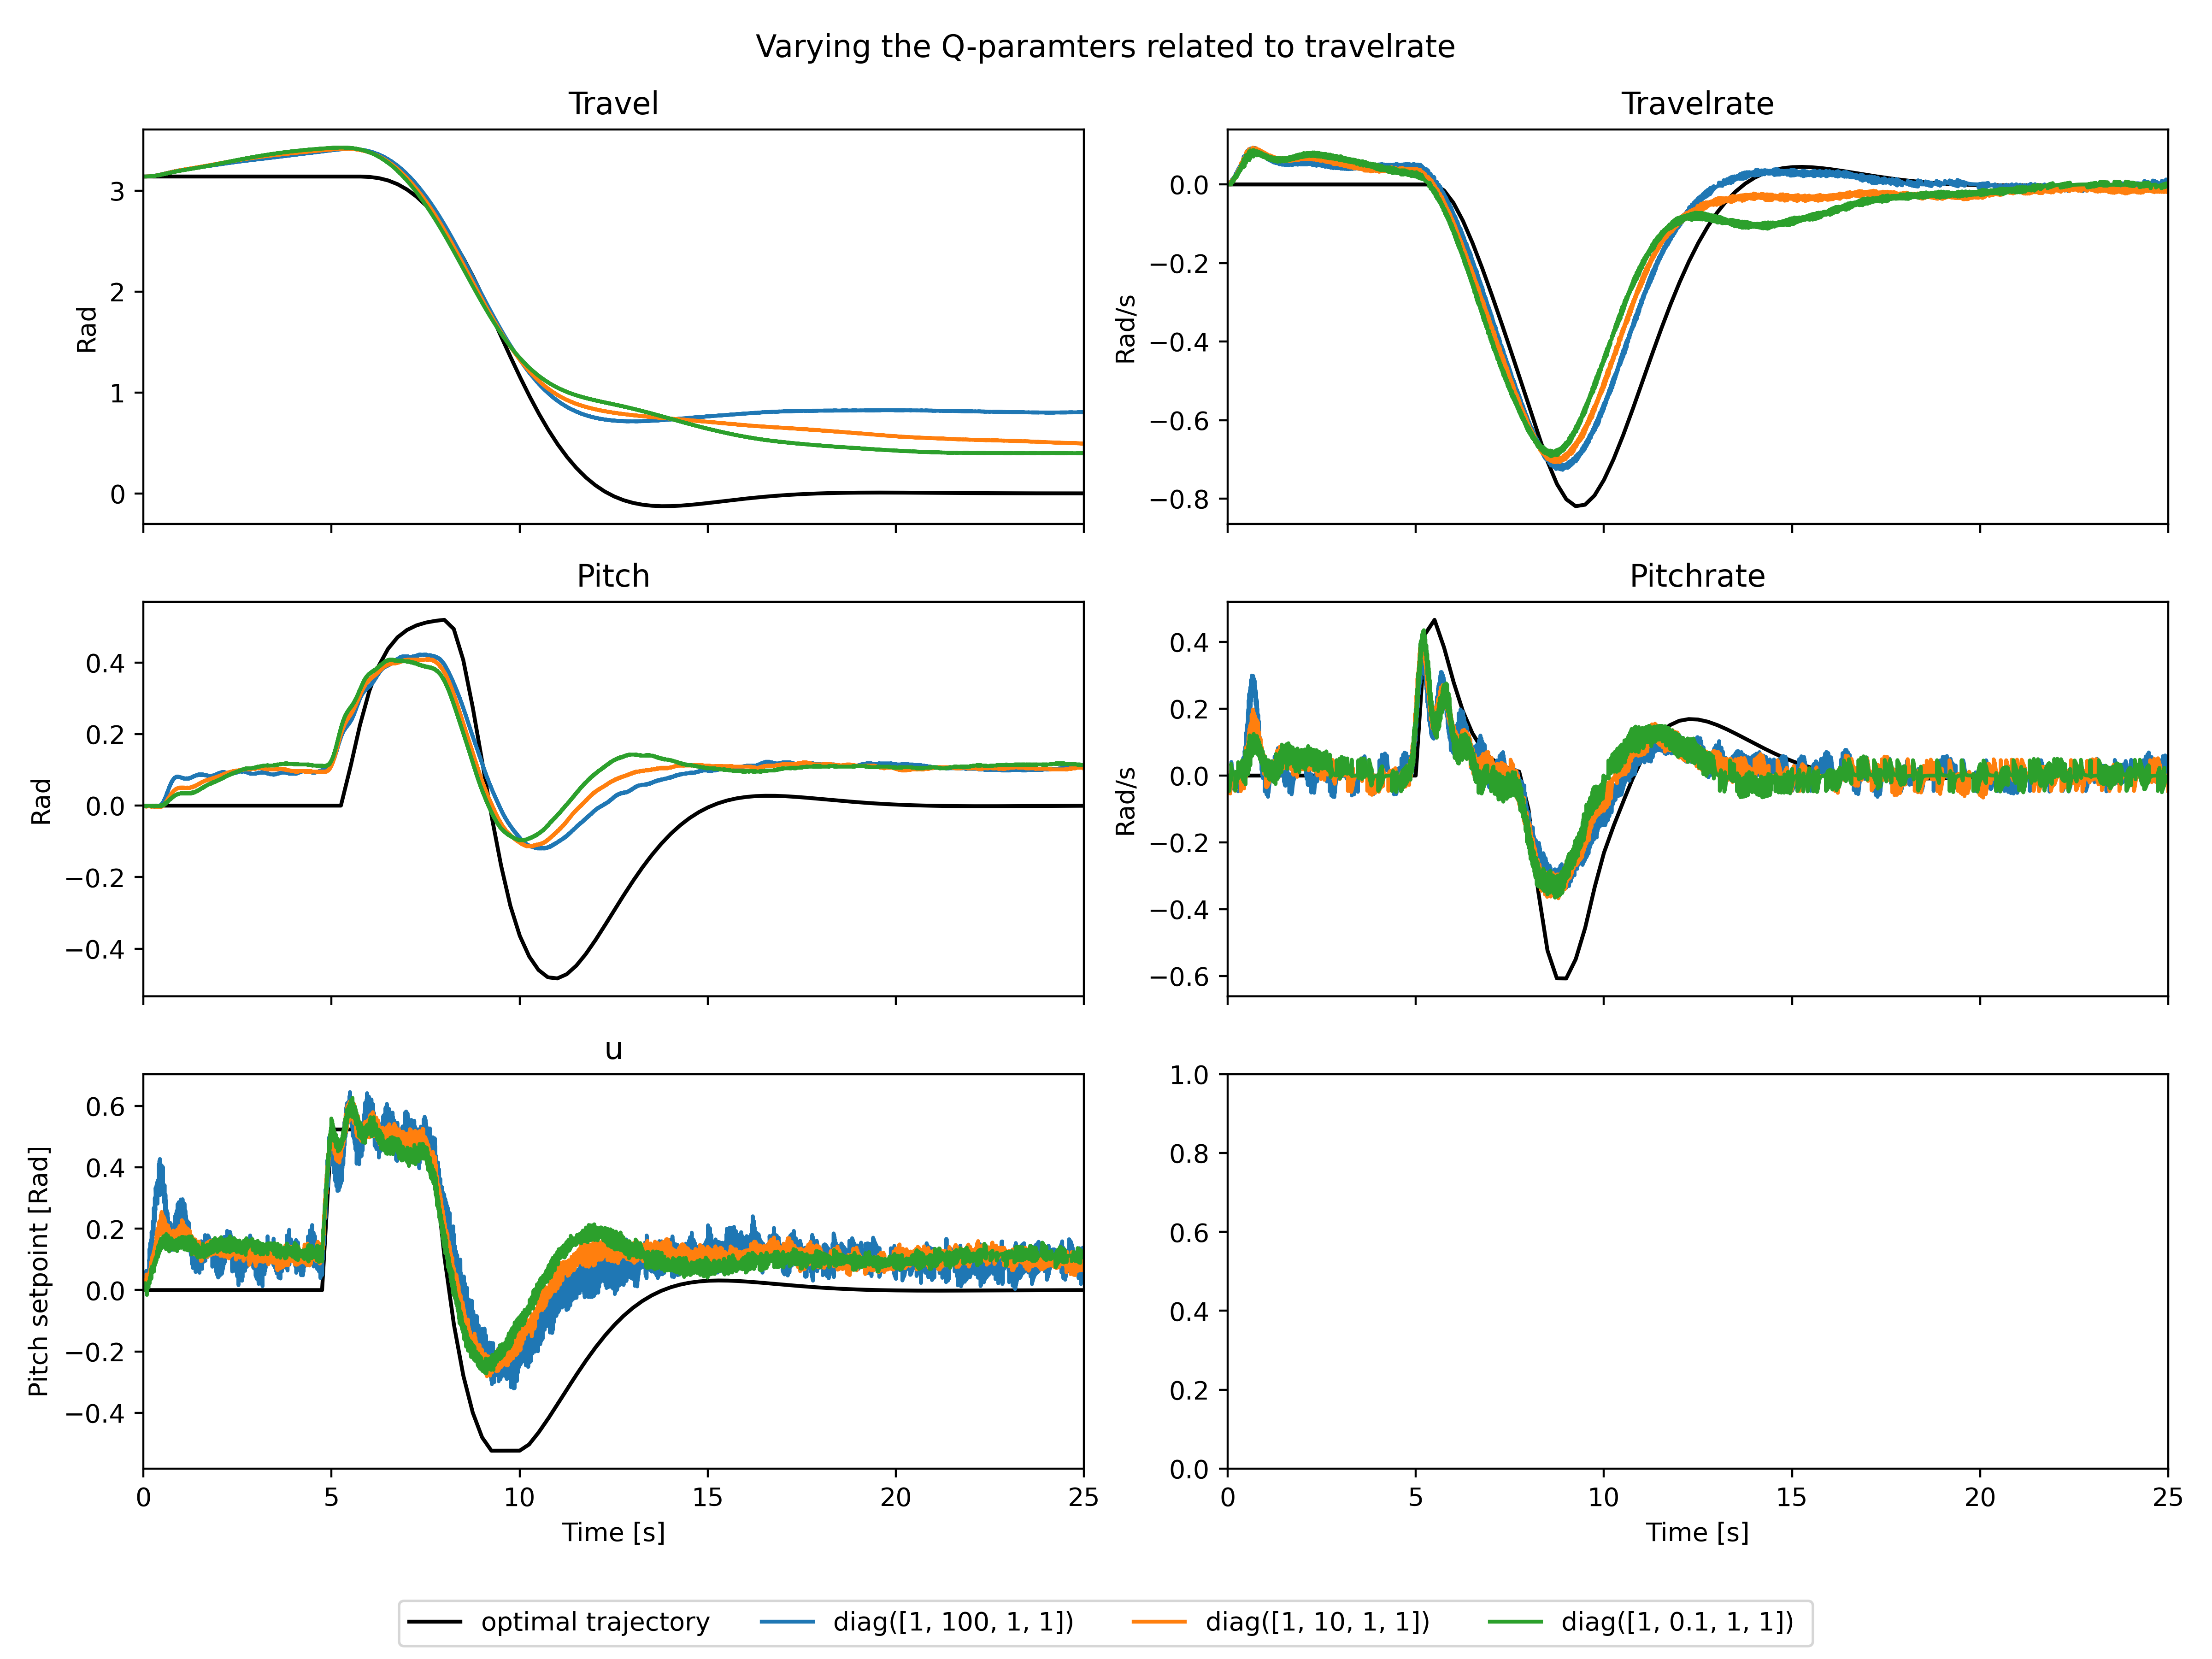
\includegraphics[width=0.8\linewidth]{figures/LAB3_Q_variations_travelrate.png}
	\caption{Changing the weight of the travelrate state, $R=1$. This had only a minor effect with small variations in the response.}
	\label{fig:LAB3_Q_variations_travelrate}
\end{figure}

\begin{figure}[h]
	\centering
	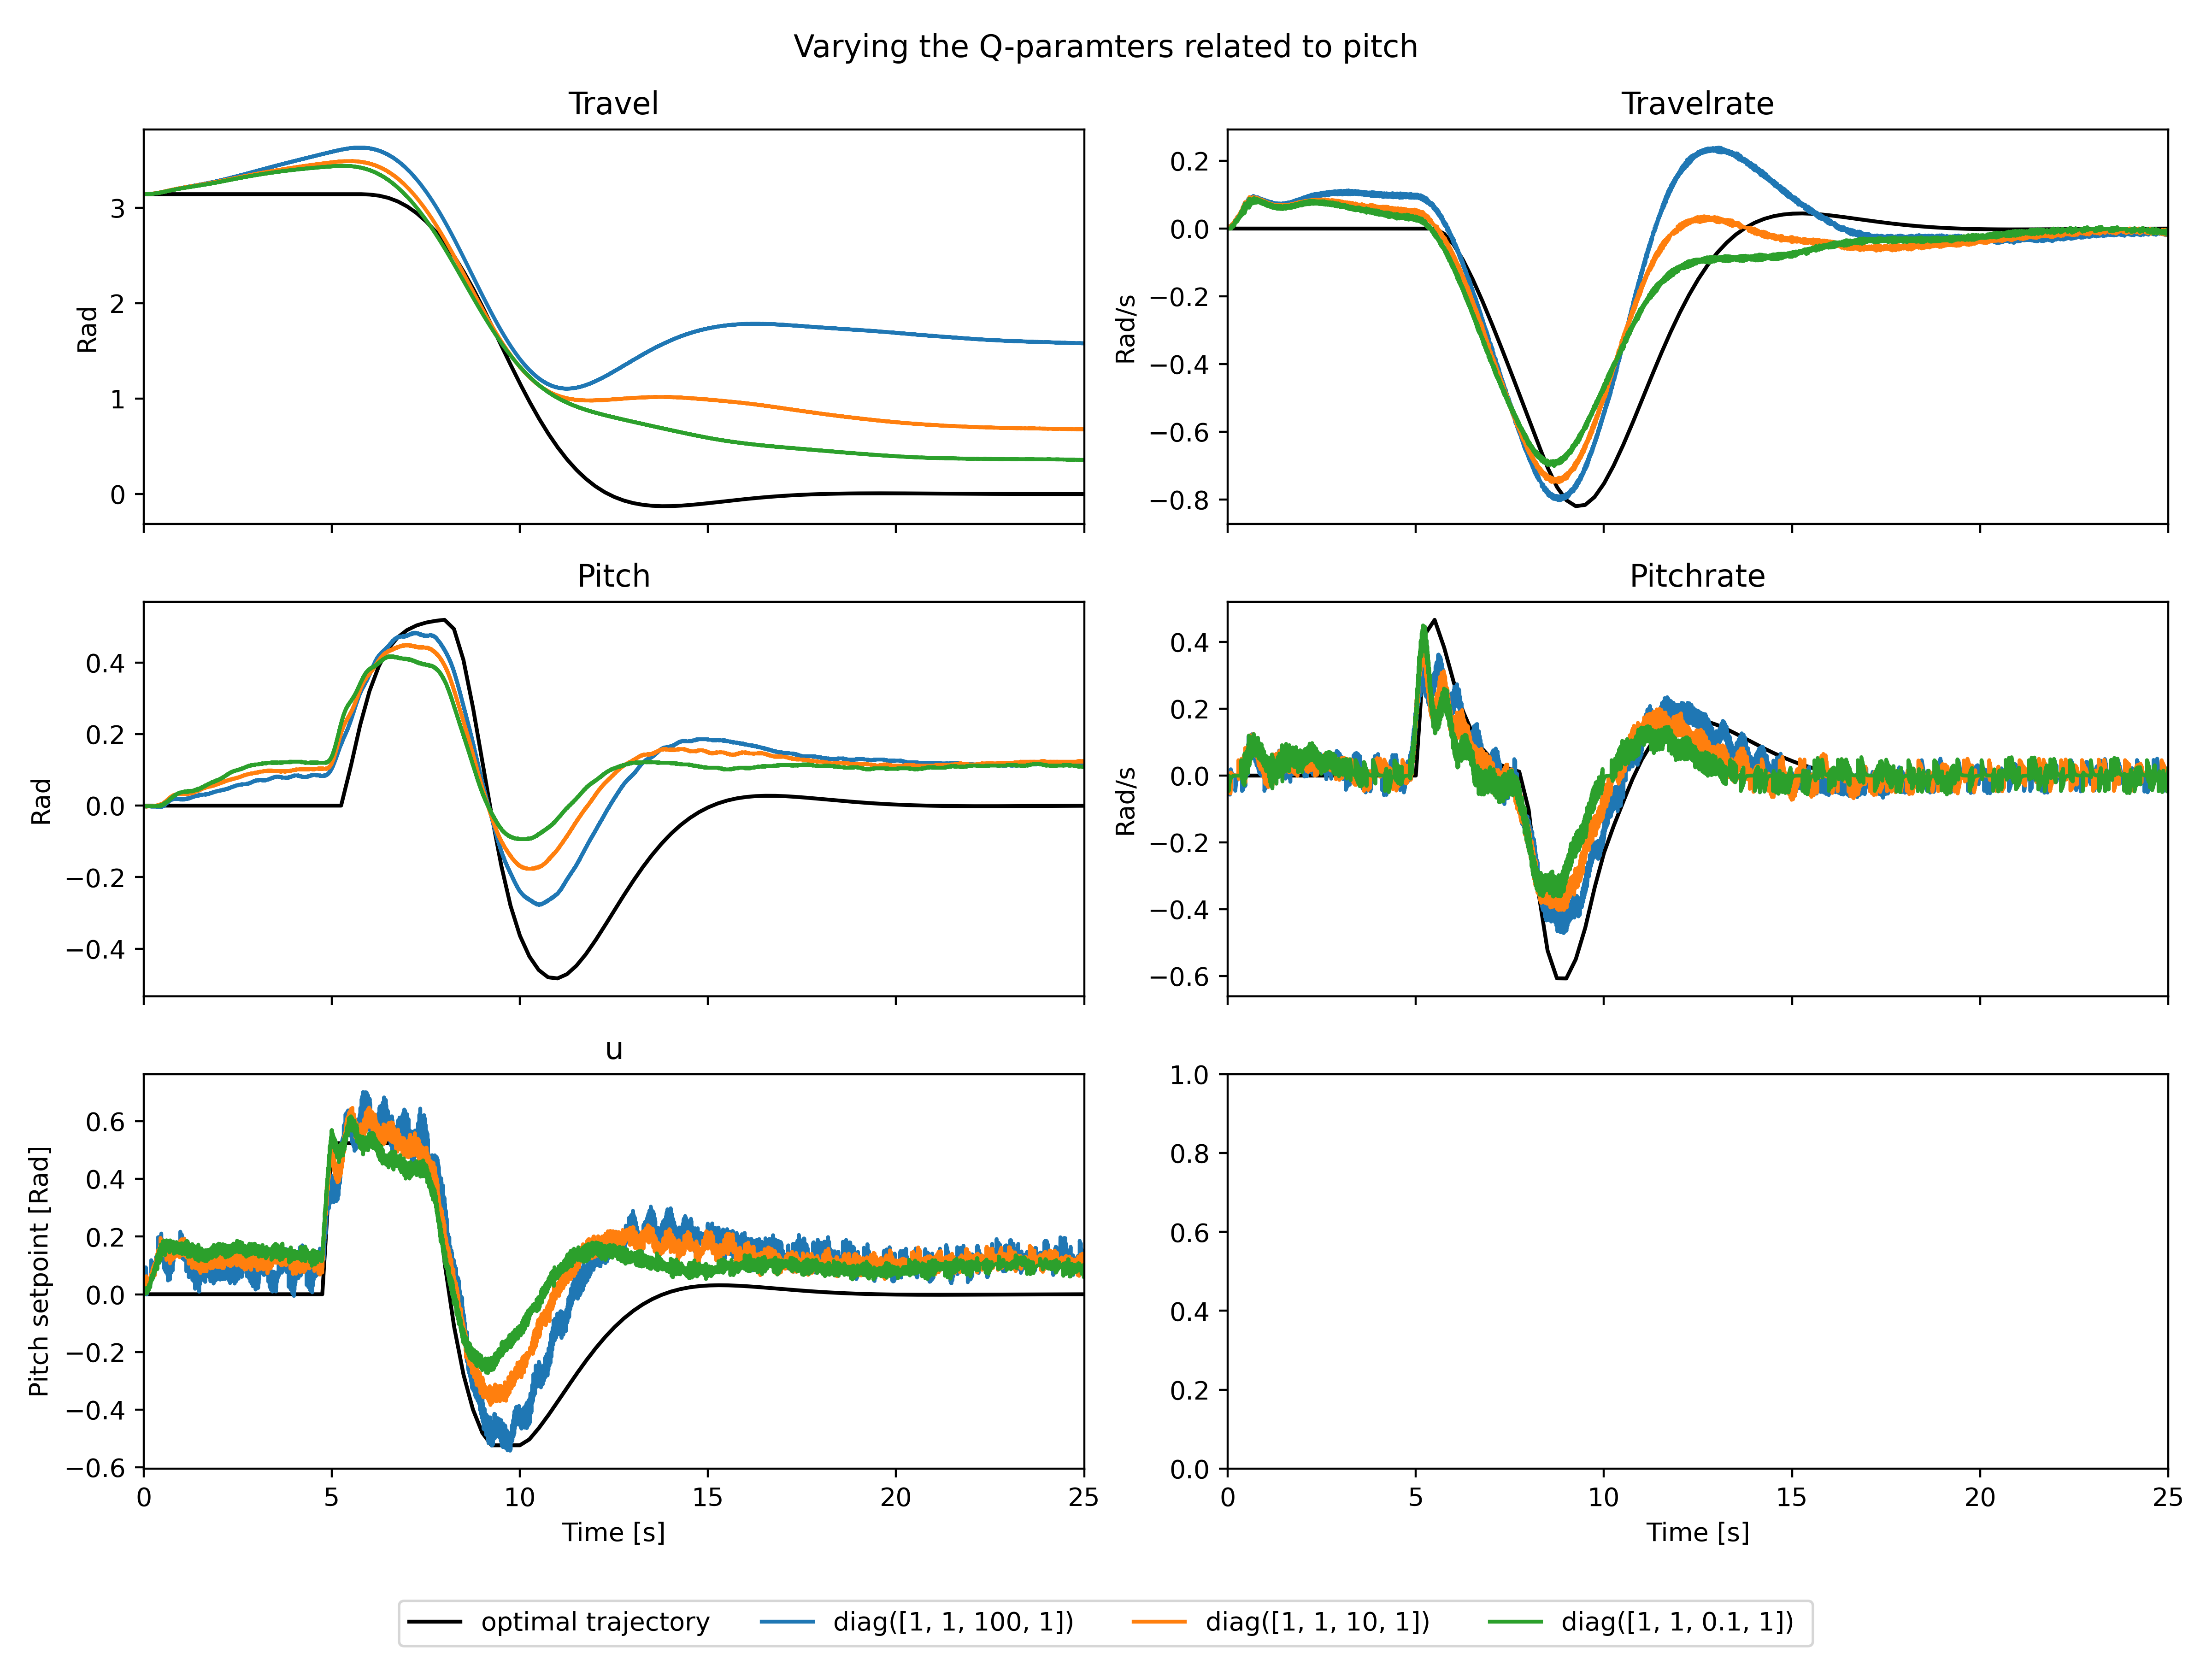
\includegraphics[width=0.8\linewidth]{figures/LAB3_Q_variations_pitch.png}
	\caption{Changing the weight of the pitch state, $R=1$. This had the effect of getting both pitch, pitch-setpoint and pitchrate closer to the planned trajectory at the expense of travel and travelrate.}
	\label{fig:LAB3_Q_variations_pitch}
\end{figure}

\begin{figure}[h]
	\centering
	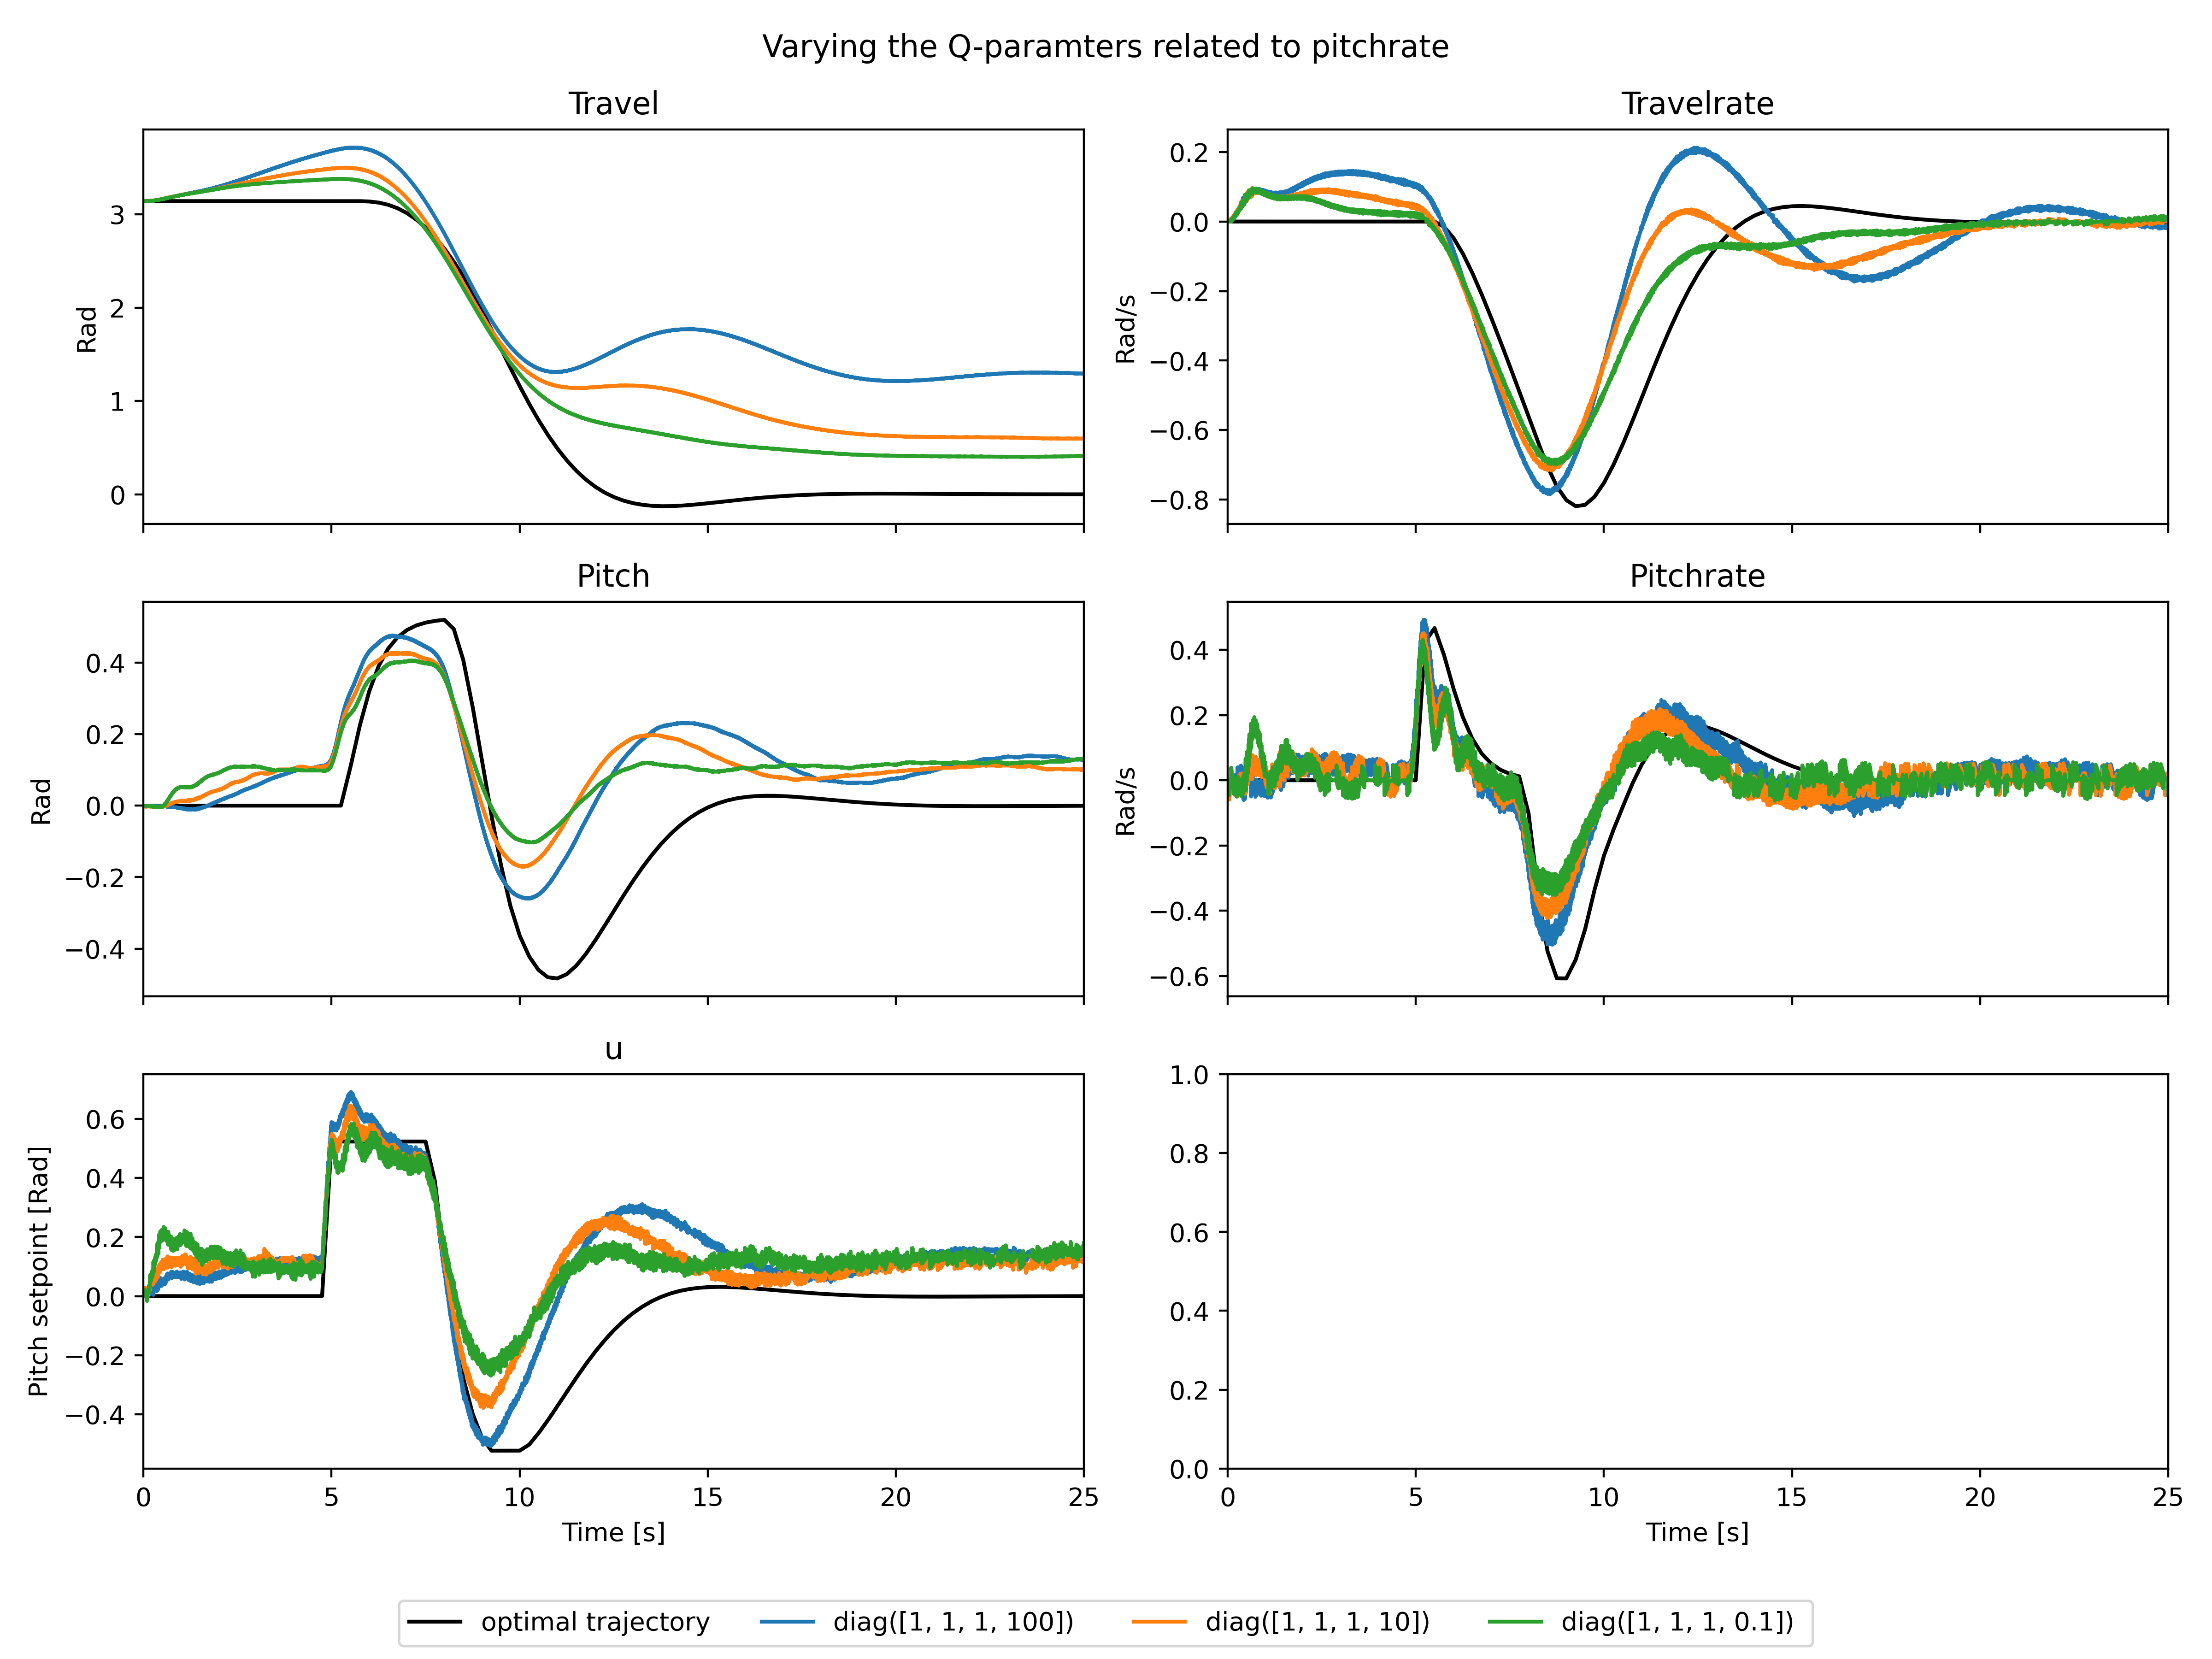
\includegraphics[width=0.8\linewidth]{figures/LAB3_Q_variations_pitchrate.png}
	\caption{Changing the weight of the pitchrate state, $R=1$. This was quite similar to \cref{fig:LAB3_Q_variations_pitch} but there is less oscillation.}
	\label{fig:LAB3_Q_variations_pitchrate}
\end{figure}

\subsubsection{Final tuning}
The final tuning prioritizes travel, as that is the most important state, while comprimizing on the gain - too low results in a large offset while too high results in too much oscillations.

\begin{figure}[h]
	\centering
	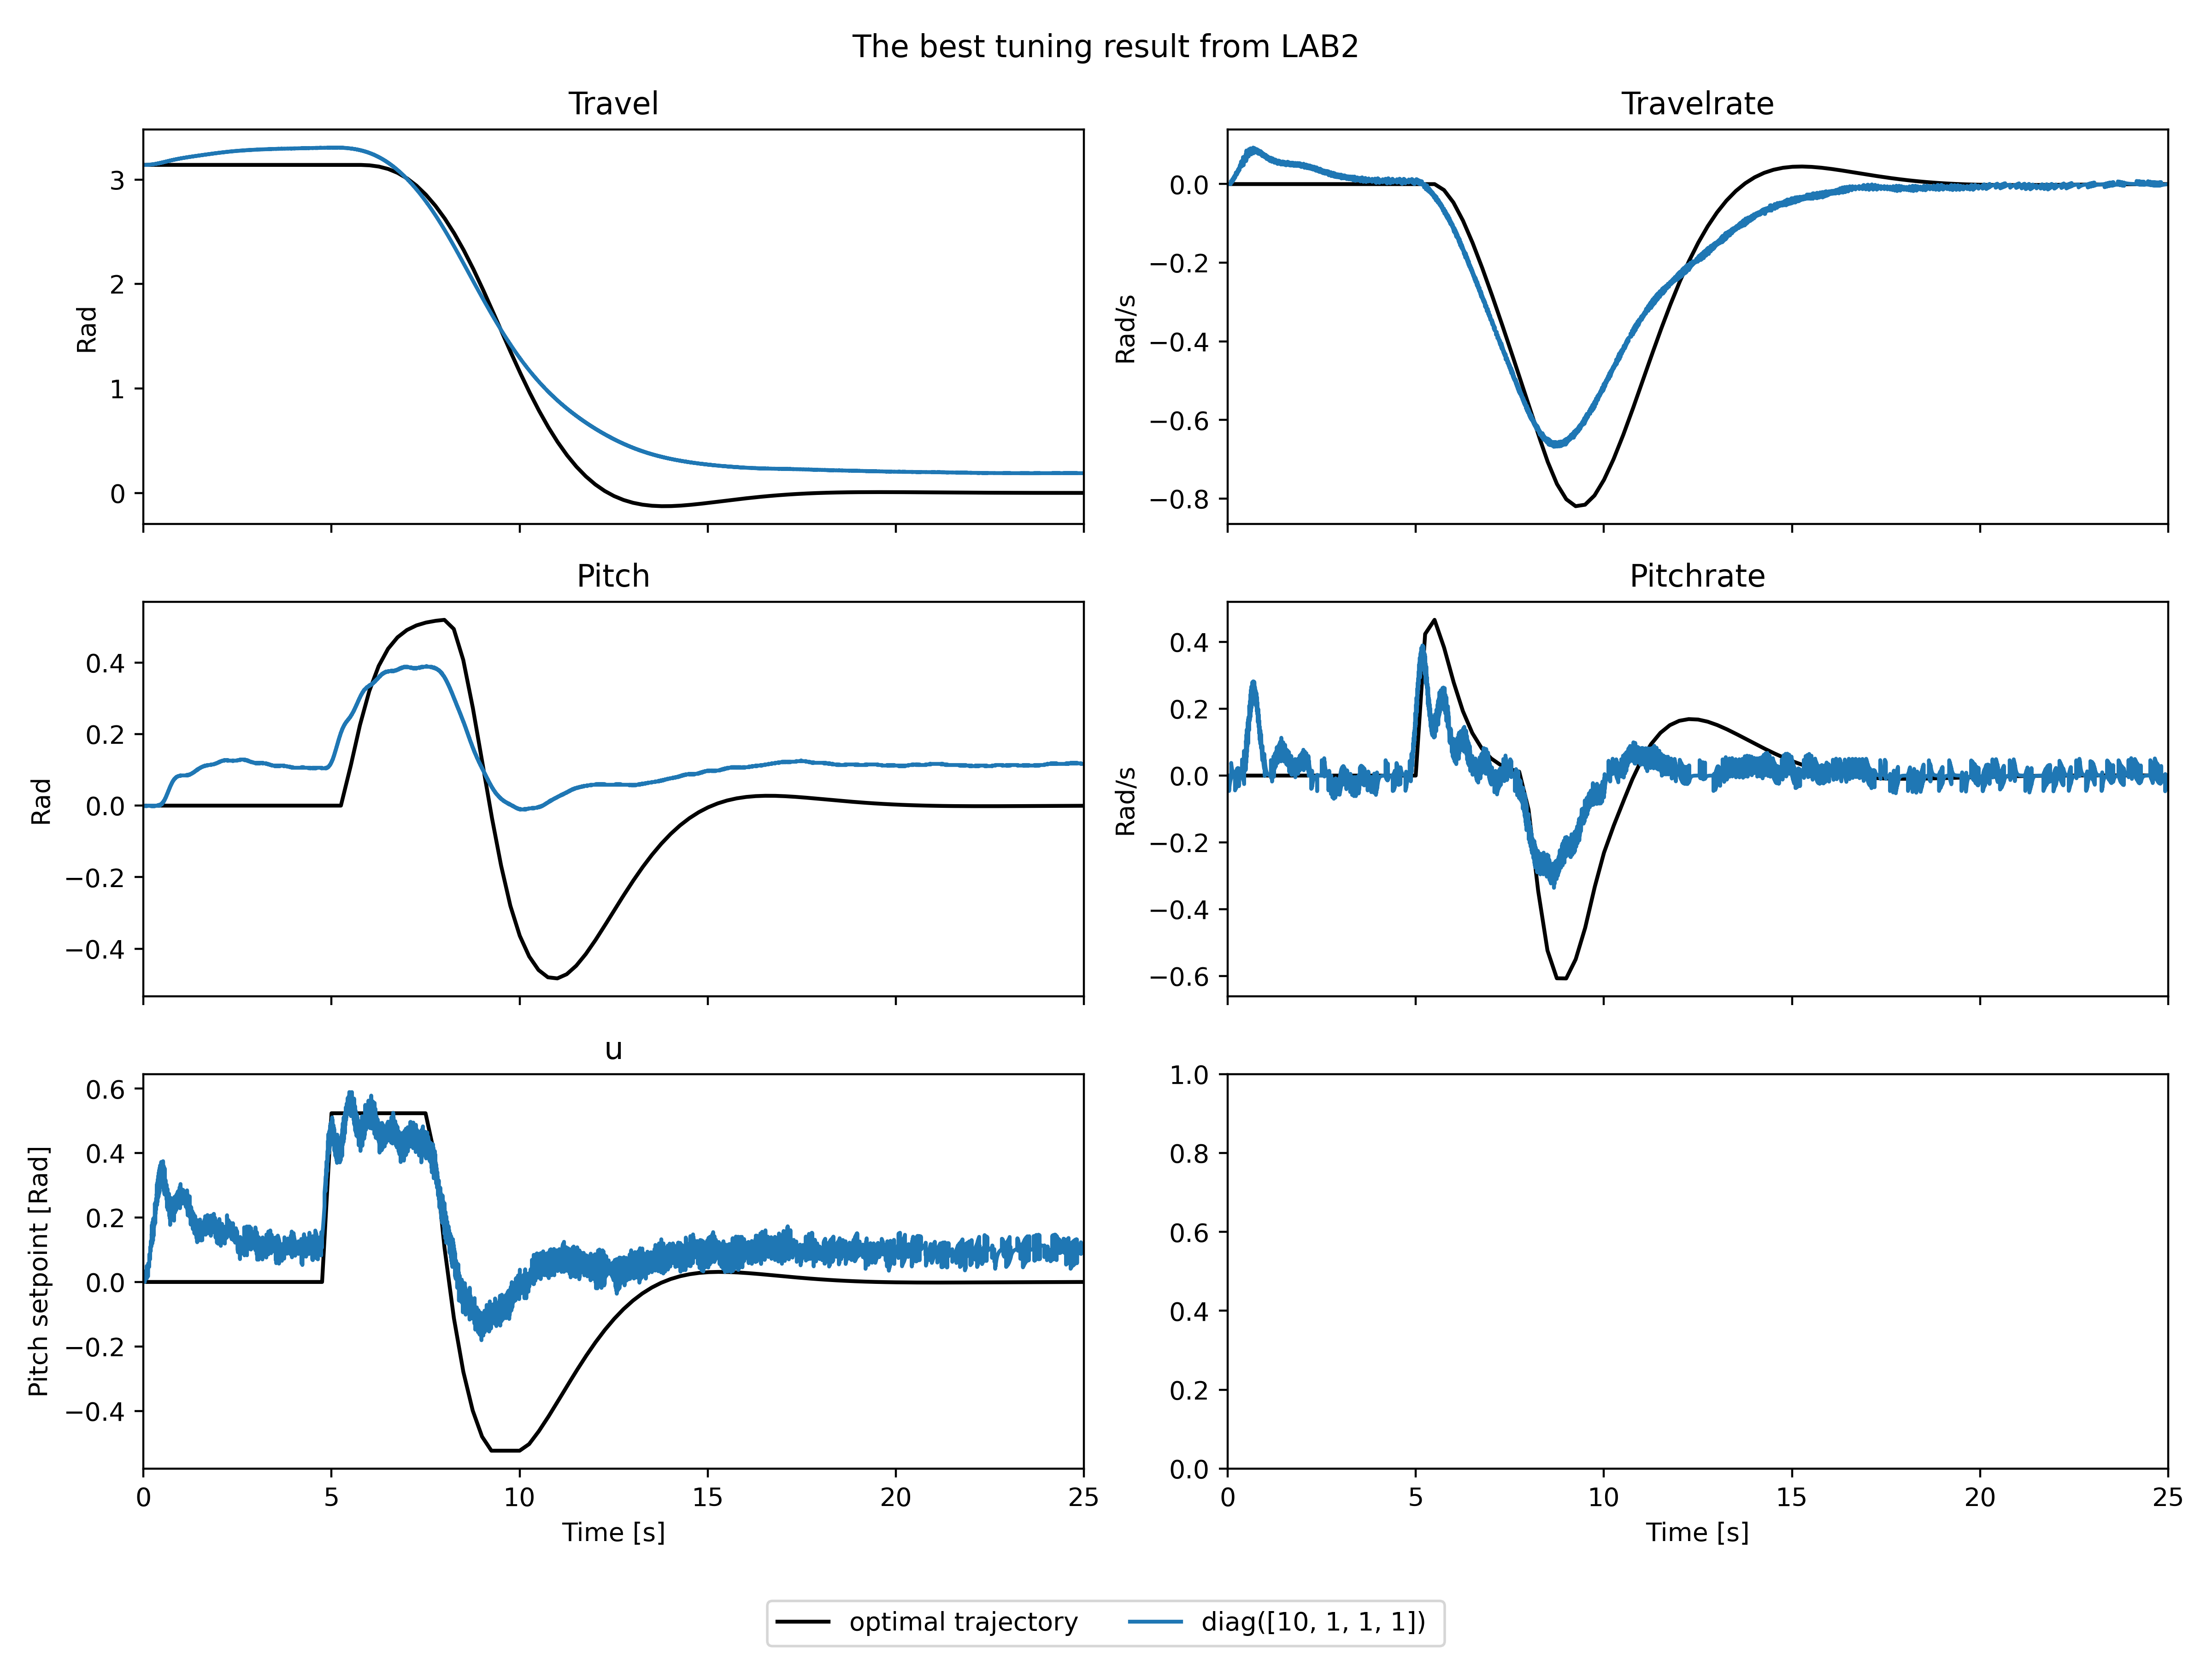
\includegraphics[width=0.8\linewidth]{figures/LAB3_best_tuning.png}
	\caption{The best tuning of LAB3. This tuning prioritizes travel with a good comprimize between high gain and oscillations.}
\end{figure}

\clearpage

\subsection{MATLAB and Simulink}
\lstinputlisting[caption= {MATLAB code for lab 3}, label={lst:lab3_matlab}]{code/problem_3.m}
\subsubsection{Simulink}
\begin{figure}[h]
	\centering
	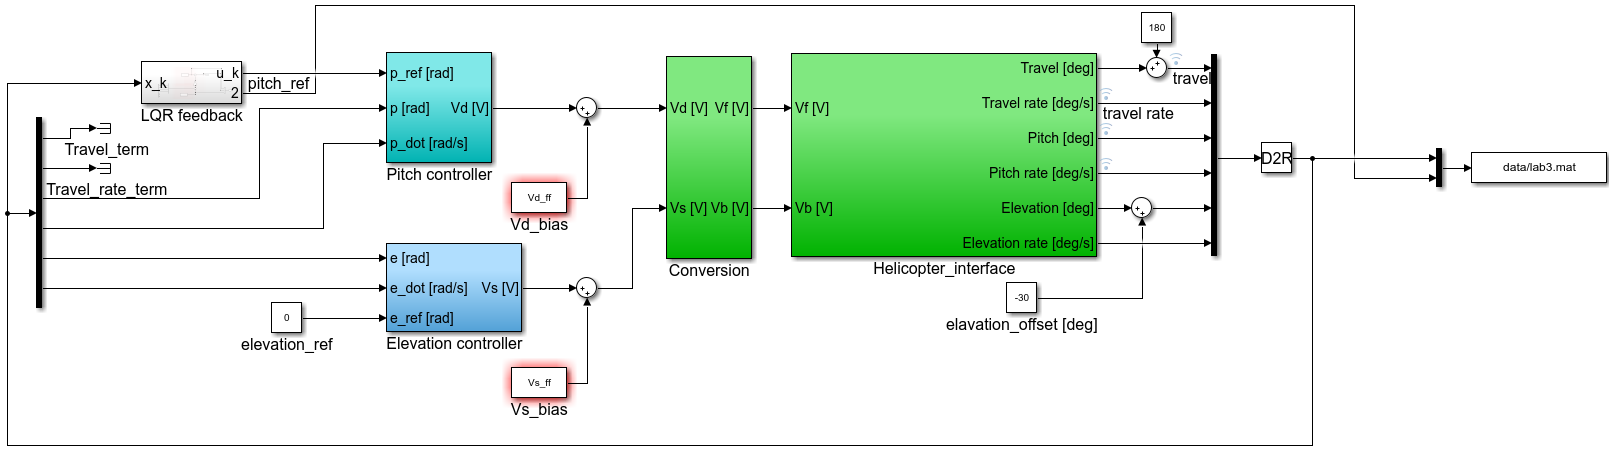
\includegraphics[width=1\linewidth, keepaspectratio]{code/lab3_simulink_1}
	\caption{Simulink diagram used in lab 3.}
	\label{fig:lab3_simulink}
\end{figure}
\begin{figure}[h]
	\centering
	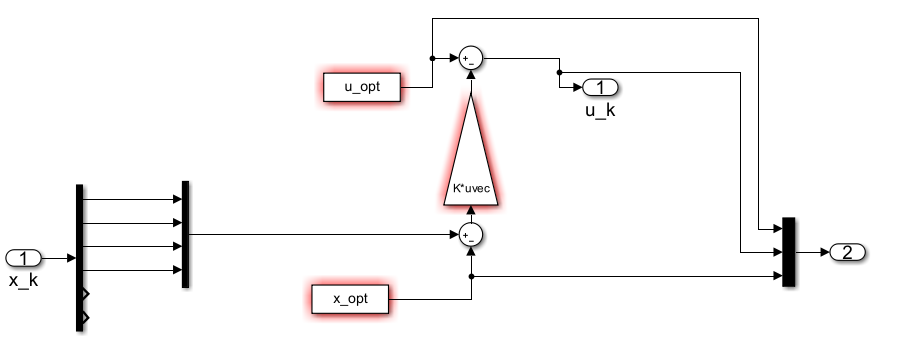
\includegraphics[width=1\linewidth, keepaspectratio]{code/lab3_simulink_2}
	\caption{``LQR Feedback'' subsystem in \cref{fig:lab3_simulink}}
	\label{fig:lab3_simulink_lqr}
\end{figure}
\end{document}
\documentclass[../main.tex]{subfiles}

\begin{document}
\section{10.4 - Optimal Control of Pitch/Travel and Elevation with Feedback}
In the previous labs the elevation has been disregarded, and assumed to be zero. In this lab, elevation is not disregarded, and the group had to calculate an optimal trajectory for the elevation as well. The criteria to be minimized was
\begin{equation}\label{eq:lab4_cost_func}
	\phi = \sum_{i=0}^{N-1} (\lambda_{i + 1} - \lambda_f)^{2} + q_1 p_{ci}^2 + q_2 e_{ci} ^2
\end{equation}
and the constraint on the elevation was:
\begin{equation}\label{eq:lab4_elevation_constraint}
	e_k \geq \alpha \text{exp}\left( -\beta (\lambda_k - \lambda_t)^2\right) \forall k \in \left\lbrace 1,...,N\right\rbrace 
\end{equation}

\subsection{The continuous model}
\textit{Answer 10.4.1.1}
The equation for elevation has been given in the problem description as
\begin{equation}\label{eq:lab4_elevation}
	\ddot{e} + K_3K_{ed}\dot{e} + K_3K_{ep}e = K_3K_{ep}e_c
\end{equation}
where $ e_c $ is the elevation setpoint.

Expanding the system defined in \cref{eq:lab2_cont_ss} to include \cref{eq:lab4_elevation}, gives a new system that includes the elevation:

\begin{equation}\label{eq:lab4_cont_ss}
	\underbrace{\begin{bmatrix}
			\dot \lambda \\
			\dot r \\
			\dot p \\
			\ddot p \\
			\dot e \\
			\ddot e \\
	\end{bmatrix}}_{\bm{\dot x}} = 
	\underbrace{
		\begin{bmatrix}
			0 & 1 & 0 & 0 & 0 & 0\\
			0 & 0 & -K_2 & 0 & 0 & 0\\
			0 & 0 & 0 & 1 & 0 & 0\\
			0 & 0 & -K_1 K_{pp} &  -K_1 K_{pd} & 0 & 0\\
			0 & 0 & 0 & 0 & 0 & 1 \\
			0 & 0 & 0 & 0 & -K_3K_{ep} & -K_3K_{ed} \\
		\end{bmatrix}
	}_{\bm A_c}
	\underbrace{
		\begin{bmatrix}
			\lambda \\ r \\ p \\ \dot{p} \\ e \\ \dot{e}
		\end{bmatrix}
	}_{\bm x}
	+
	\underbrace{
		\begin{bmatrix}
			0 & 0 \\
			0 & 0\\
			0 & 0\\
			K_1 K_{pp} & 0\\
			0 & 0 \\
			0 & K_3K_{ep} \\
		\end{bmatrix}
	}_{\bm B_c} 
	\underbrace{
		\begin{bmatrix}
			p_c \\
			e_c \\
		\end{bmatrix}
	}_{\bm u}
\end{equation}

\subsection{The discretized model}
\textit{Answer 10.4.1.2}
Discretizing the continuous system defined in \cref{eq:lab4_cont_ss} was done using the forward Euler method (see \cref{sec:lab2_disc} for more information about this method).

The resulting dicretized system became: 
\begin{equation}\label{eq:lab4_disc_ss}
	\bm A_d = \begin{bmatrix}
		1 & T & 0 & 0 & 0 & 0\\
		0 & 1 & -TK_2 & 0 & 0 & 0\\
		0 & 0 & 1 & T & 0 & 0\\
		0 & 0 & -T K_1 K_{pp} &  1 - T K_1 K_{pd} & 0 & 0\\
		0 & 0 & 0 & 0 & 1 & T \\
		0 & 0 & 0 & 0 & -T K_3 K_{ep} & 1 - TK_3K_{ed} \\
	\end{bmatrix}, \quad
	\bm B_d = \begin{bmatrix}
		0 & 0 \\
		0 & 0\\
		0 & 0\\
		T K_1 K_{pp} & 0\\
		0 & 0 \\
		0 & T K_3K_{ep} \\
	\end{bmatrix}
\end{equation}
where $ T $ is the sample-time.

\subsection{Experimental results}
\textit{Printouts of data from relevant experiments (plots).
Discussion and analysis of the results.
Answer 10.4.2.6 here.}

The group's goal was as in the other labs, to make the helicopter follow the optimal trajectory to $ \lambda_f $ as close as possible. Making the helicopter follow the trajectory consisted of two parts: 
\begin{enumerate}
	\item Tune the LQ regulator to get a good feedback-gain matrix.
	\item Find an optimal trajectory the helicopter could follow.
\end{enumerate}

\subsubsection{Tuning LQ regulator}
Before the group started testing the helicopter's response optimal trajectory found using the SQP-algorithm, the LQ regulator used to find the feedback-gain matrix $\bm K$ had to be tuned. The LQ regulator was exactly the same as the one describe in \cref{kap:task_10_3_LQ_controller}, but now with expanded state and input as described in \cref{eq:lab4_cont_ss}. This means that $ \bm Q $ was now a diagonal matrix of size 6x6, and $ \bm R $ was a diagonal matrix of 2x2. Tuning the LQ regulator is a vital part of achieving as good response. Since the elevation is decoupled from the rest of the states, it should been possible to use the tuning from \cref{sec:lab3_result} and find a good tuning for the elevation (i.e. tuning Q(5,5), Q(6,6) and R(2, 2)). However, in reality the helicopter's state is not decoupled (see \cref{sec:lab4_decoupled}), so to achieve good tuning the group had to tune the whole system again.

A good rule of thumb is that the LQ regulator should be tuned with an input trajectory that one know the helicopter actually can follow. If the helicopter has an input trajectory that is physical impossible to achieve, the tuning will become hard. Therefore, the group tried to create a moderate input-trajectory which seemed reasonable based on their experience from the lab. However, the task was harder than anticipated, and the group did not have enough time to do this. 

Since the group was not able to make a tuning-trajectory for the states and inputs, an optimal trajectory from solving the optimization problem using $q_1 = q_2 = 1$ in the cost function, was used as a replacement. This gave the optimal trajectories shown in \cref{fig:lab4_opt_trajectory}

\begin{figure}[h]
	\centering
	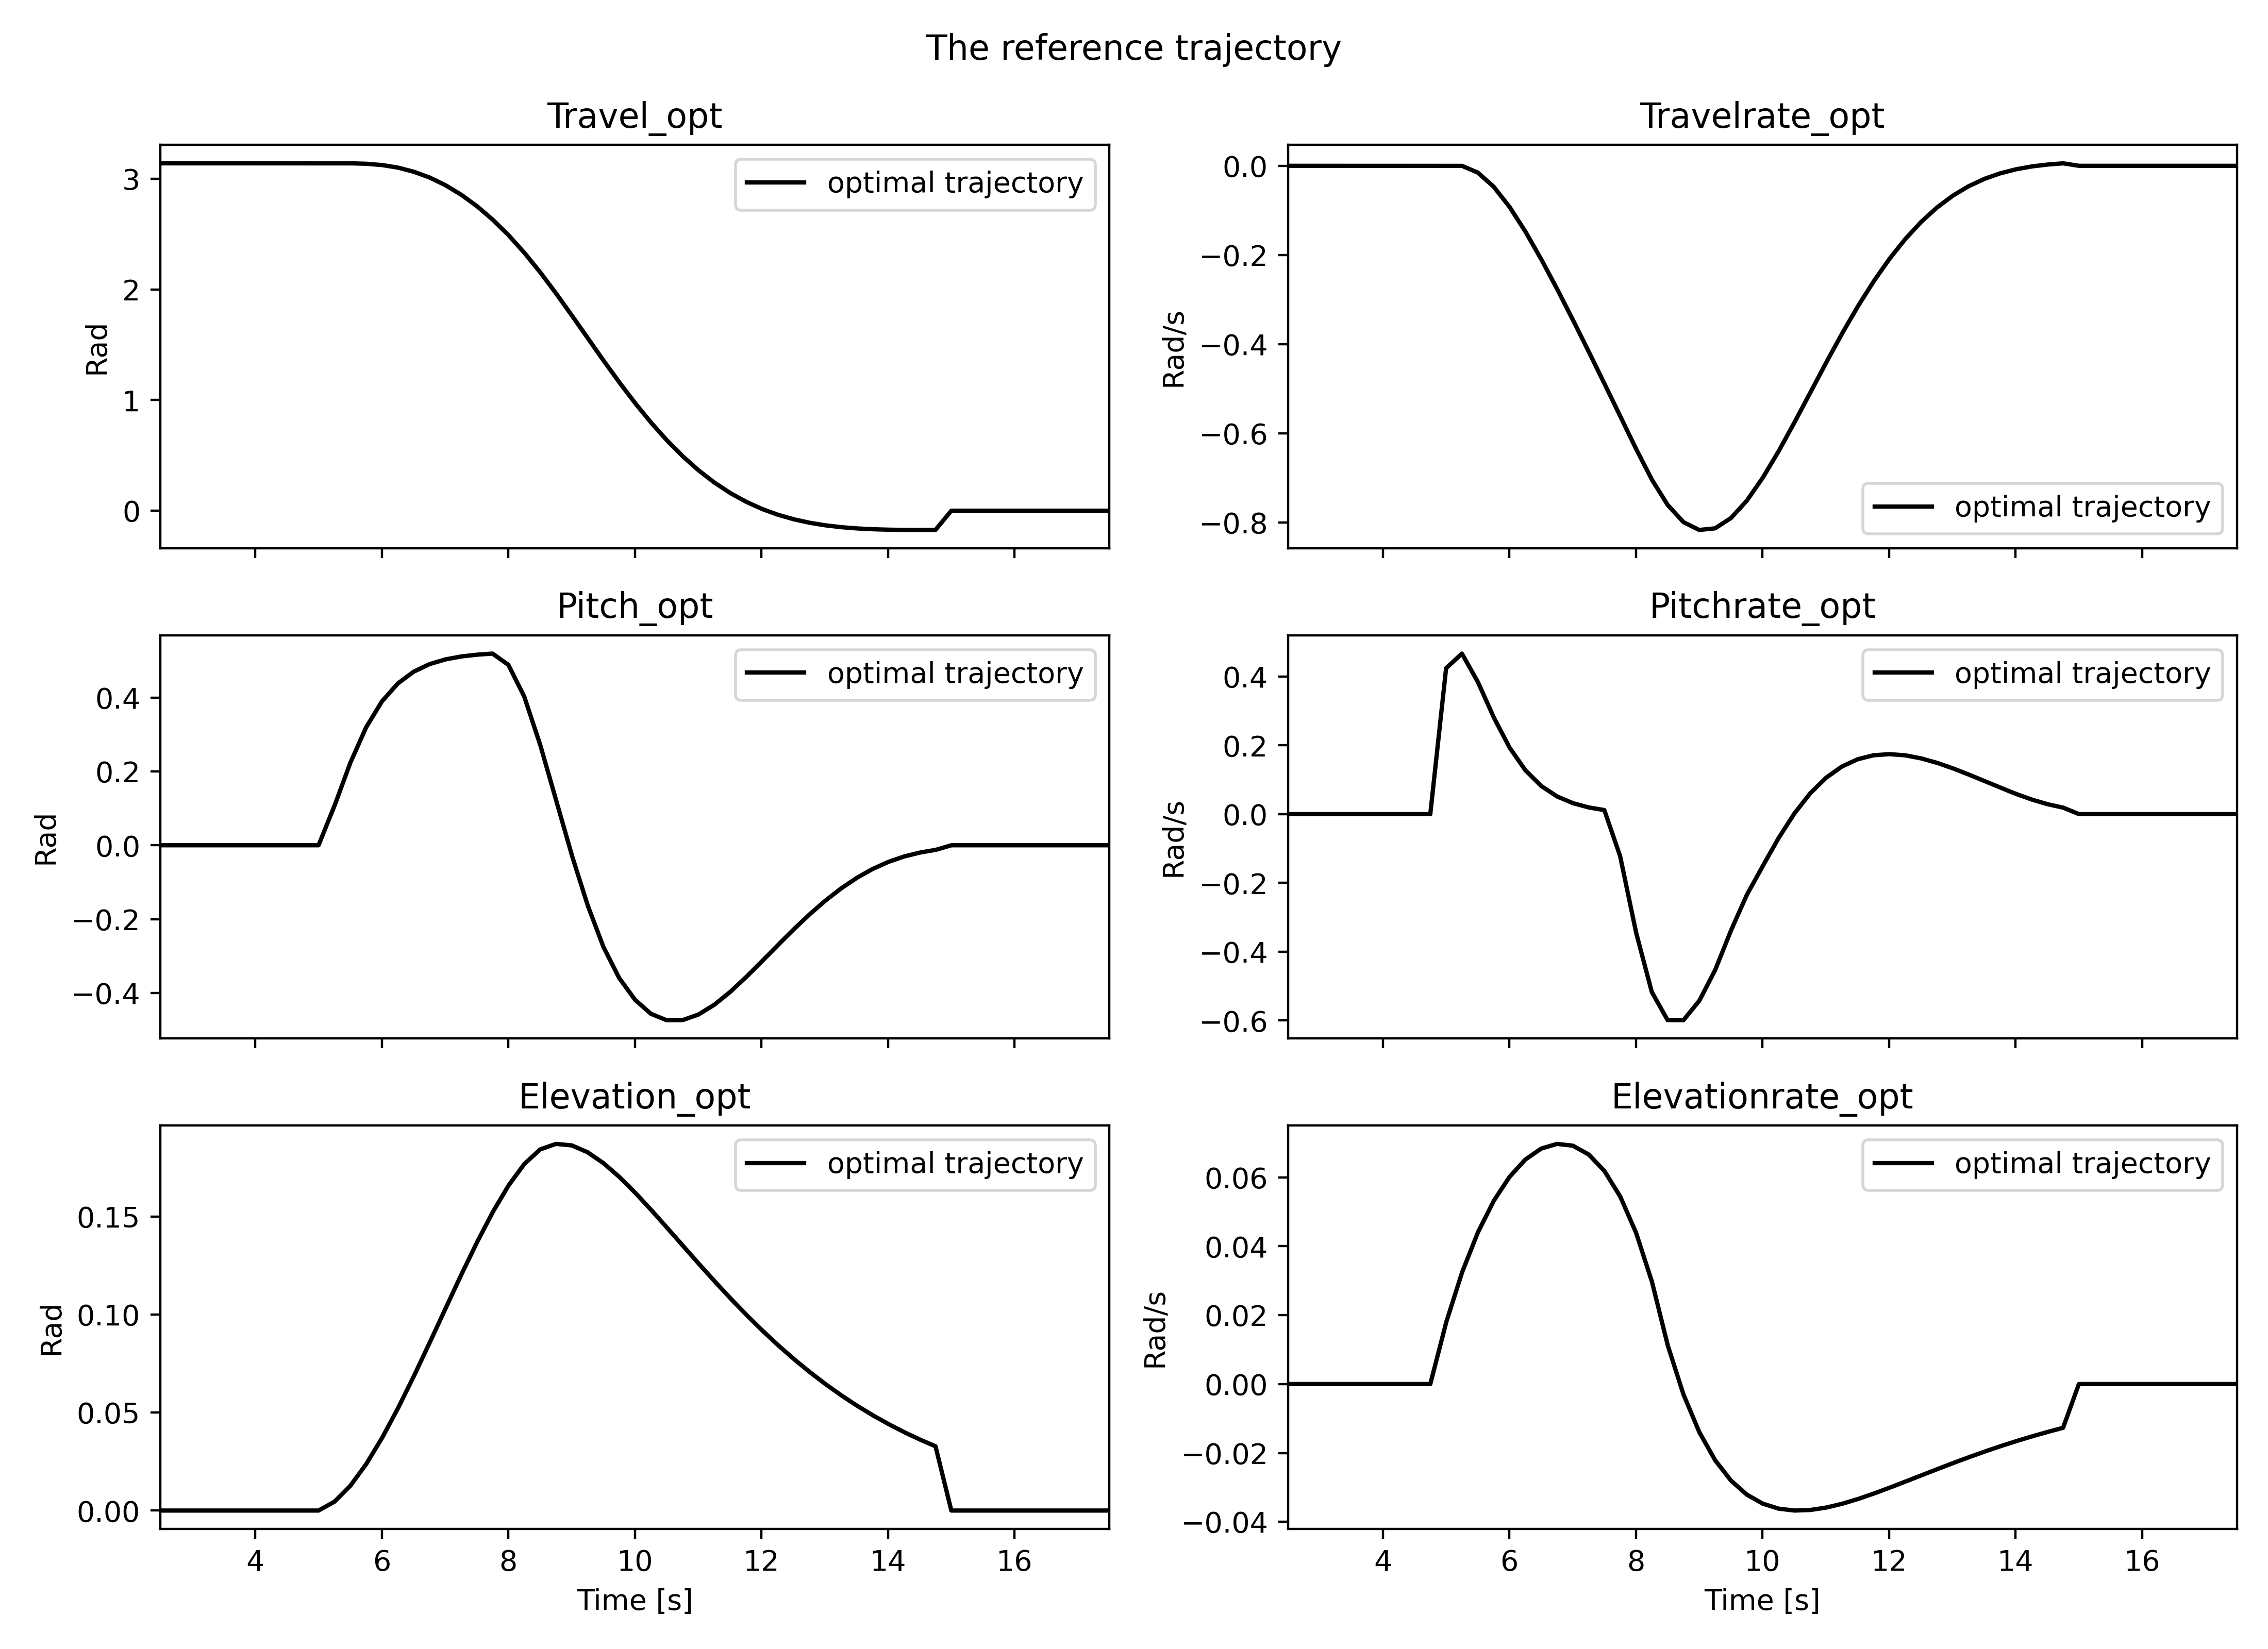
\includegraphics[width=\linewidth]{figures/LAB4_reference_trajectory.png}
	\caption{Optimal trajectories using  $q_1 = q_2 = 1$ in the cost function.}
\end{figure}

In the tuning process we decided to keep $ \bm R $ and $ \bm Q $ as diagonal matrices. $ \bm R $ was set constant equal the identity matrix, i.e. $\bm R = \bm I_2$. The diagonal elements of $ \bm Q $ was then changed to get a good tuning. As in \todo{cref lab3 lqr tuning}each diagonal entry in Q corresponds to the corresponding state in \cref{eq:lab4_cont_ss} \todo{REFORMULATE}. This makes the tuning process simpler since a change in an entry $ \bm Q $ has an expected impact on the response. Higher values of $ \bm Q $ results in inputs with larger magnitude, which again gives a faster response. Having too small values on the diagonal of $ \bm Q $ will therefor give a slow response. Having too large values on the diagonal of $ \bm Q $ will also have unwanted effects as the helicopter approaches a less stable tuning. This is shown in \cref{fig:lab4_diff_Q_values} where the low valued $ \bm Q $ gives a slower response, and a higher valued $ \bm Q $ gives an oscillating response (especially for the pitch rate). The oscillations are noticeable in th ereal world as a shaking helicopter.
\begin{figure}[h]
	\centering
	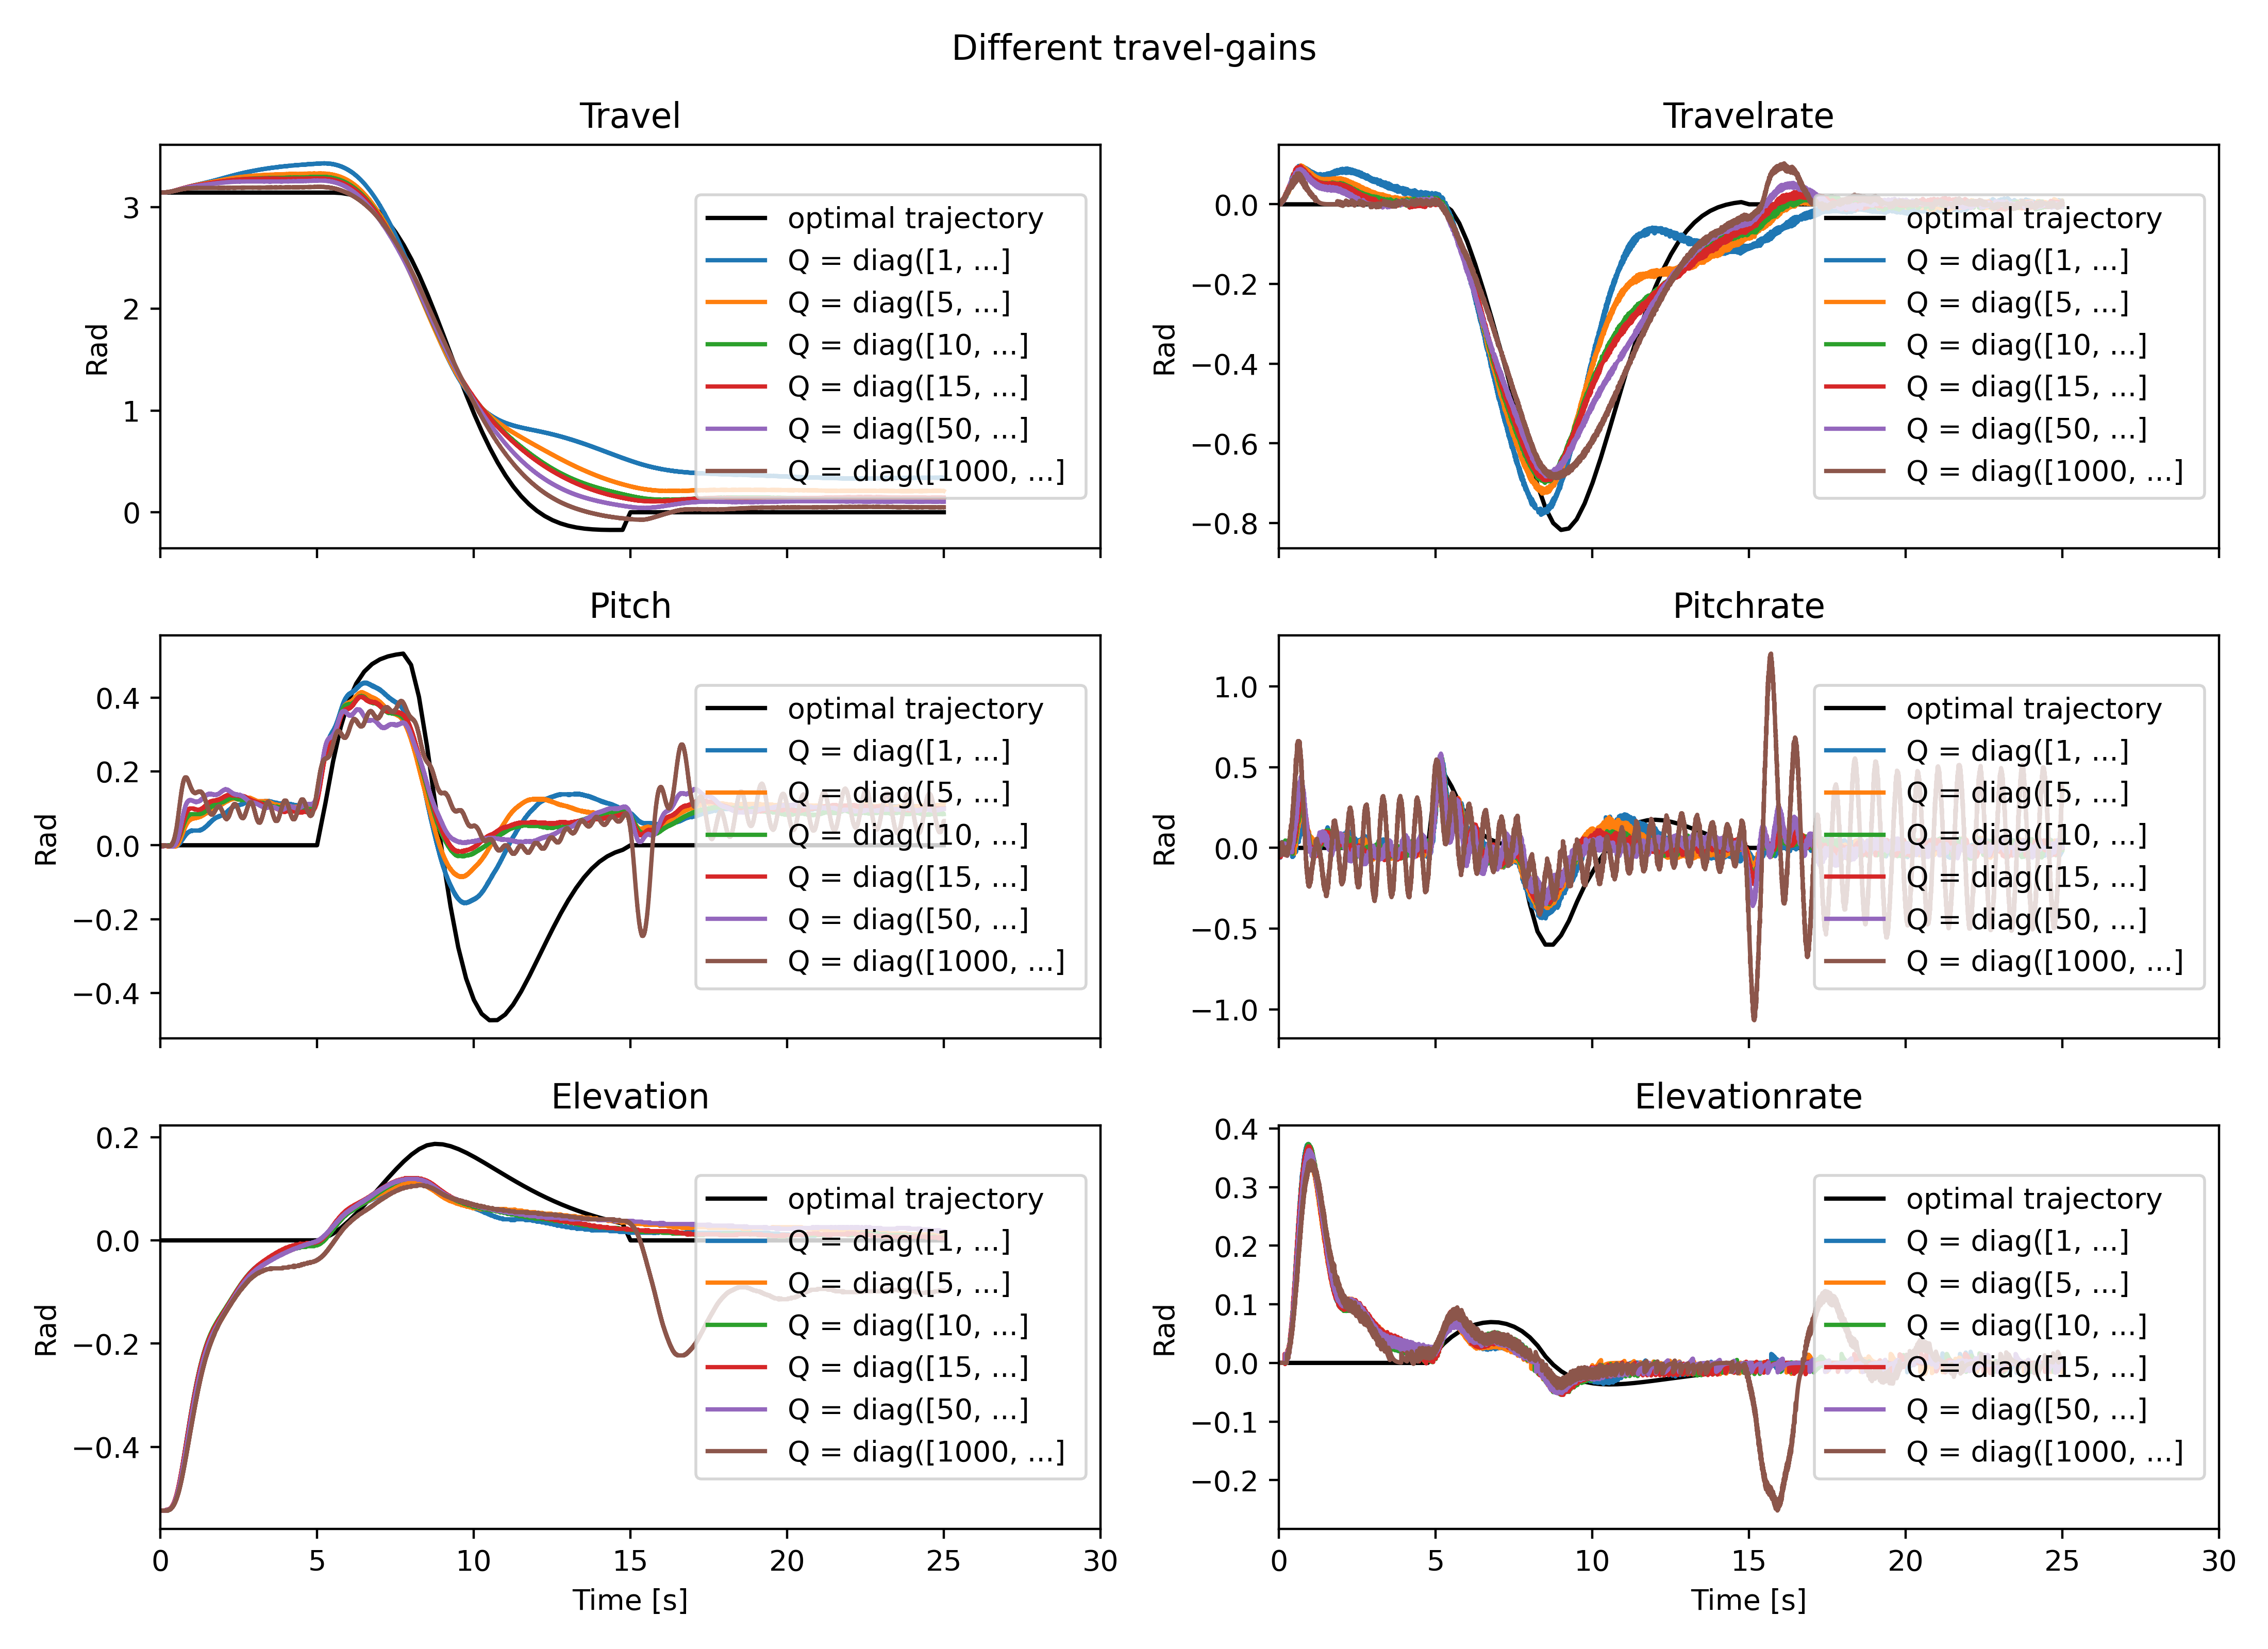
\includegraphics[width=\linewidth]{figures/LAB4_travel_gains.png}
	\caption{Her er alle verdiene vi brukte, bør nok rydde opp litt.}
	\label{fig:lab4_diff_Q_values}
\end{figure}

\begin{figure}[h]
	\centering
	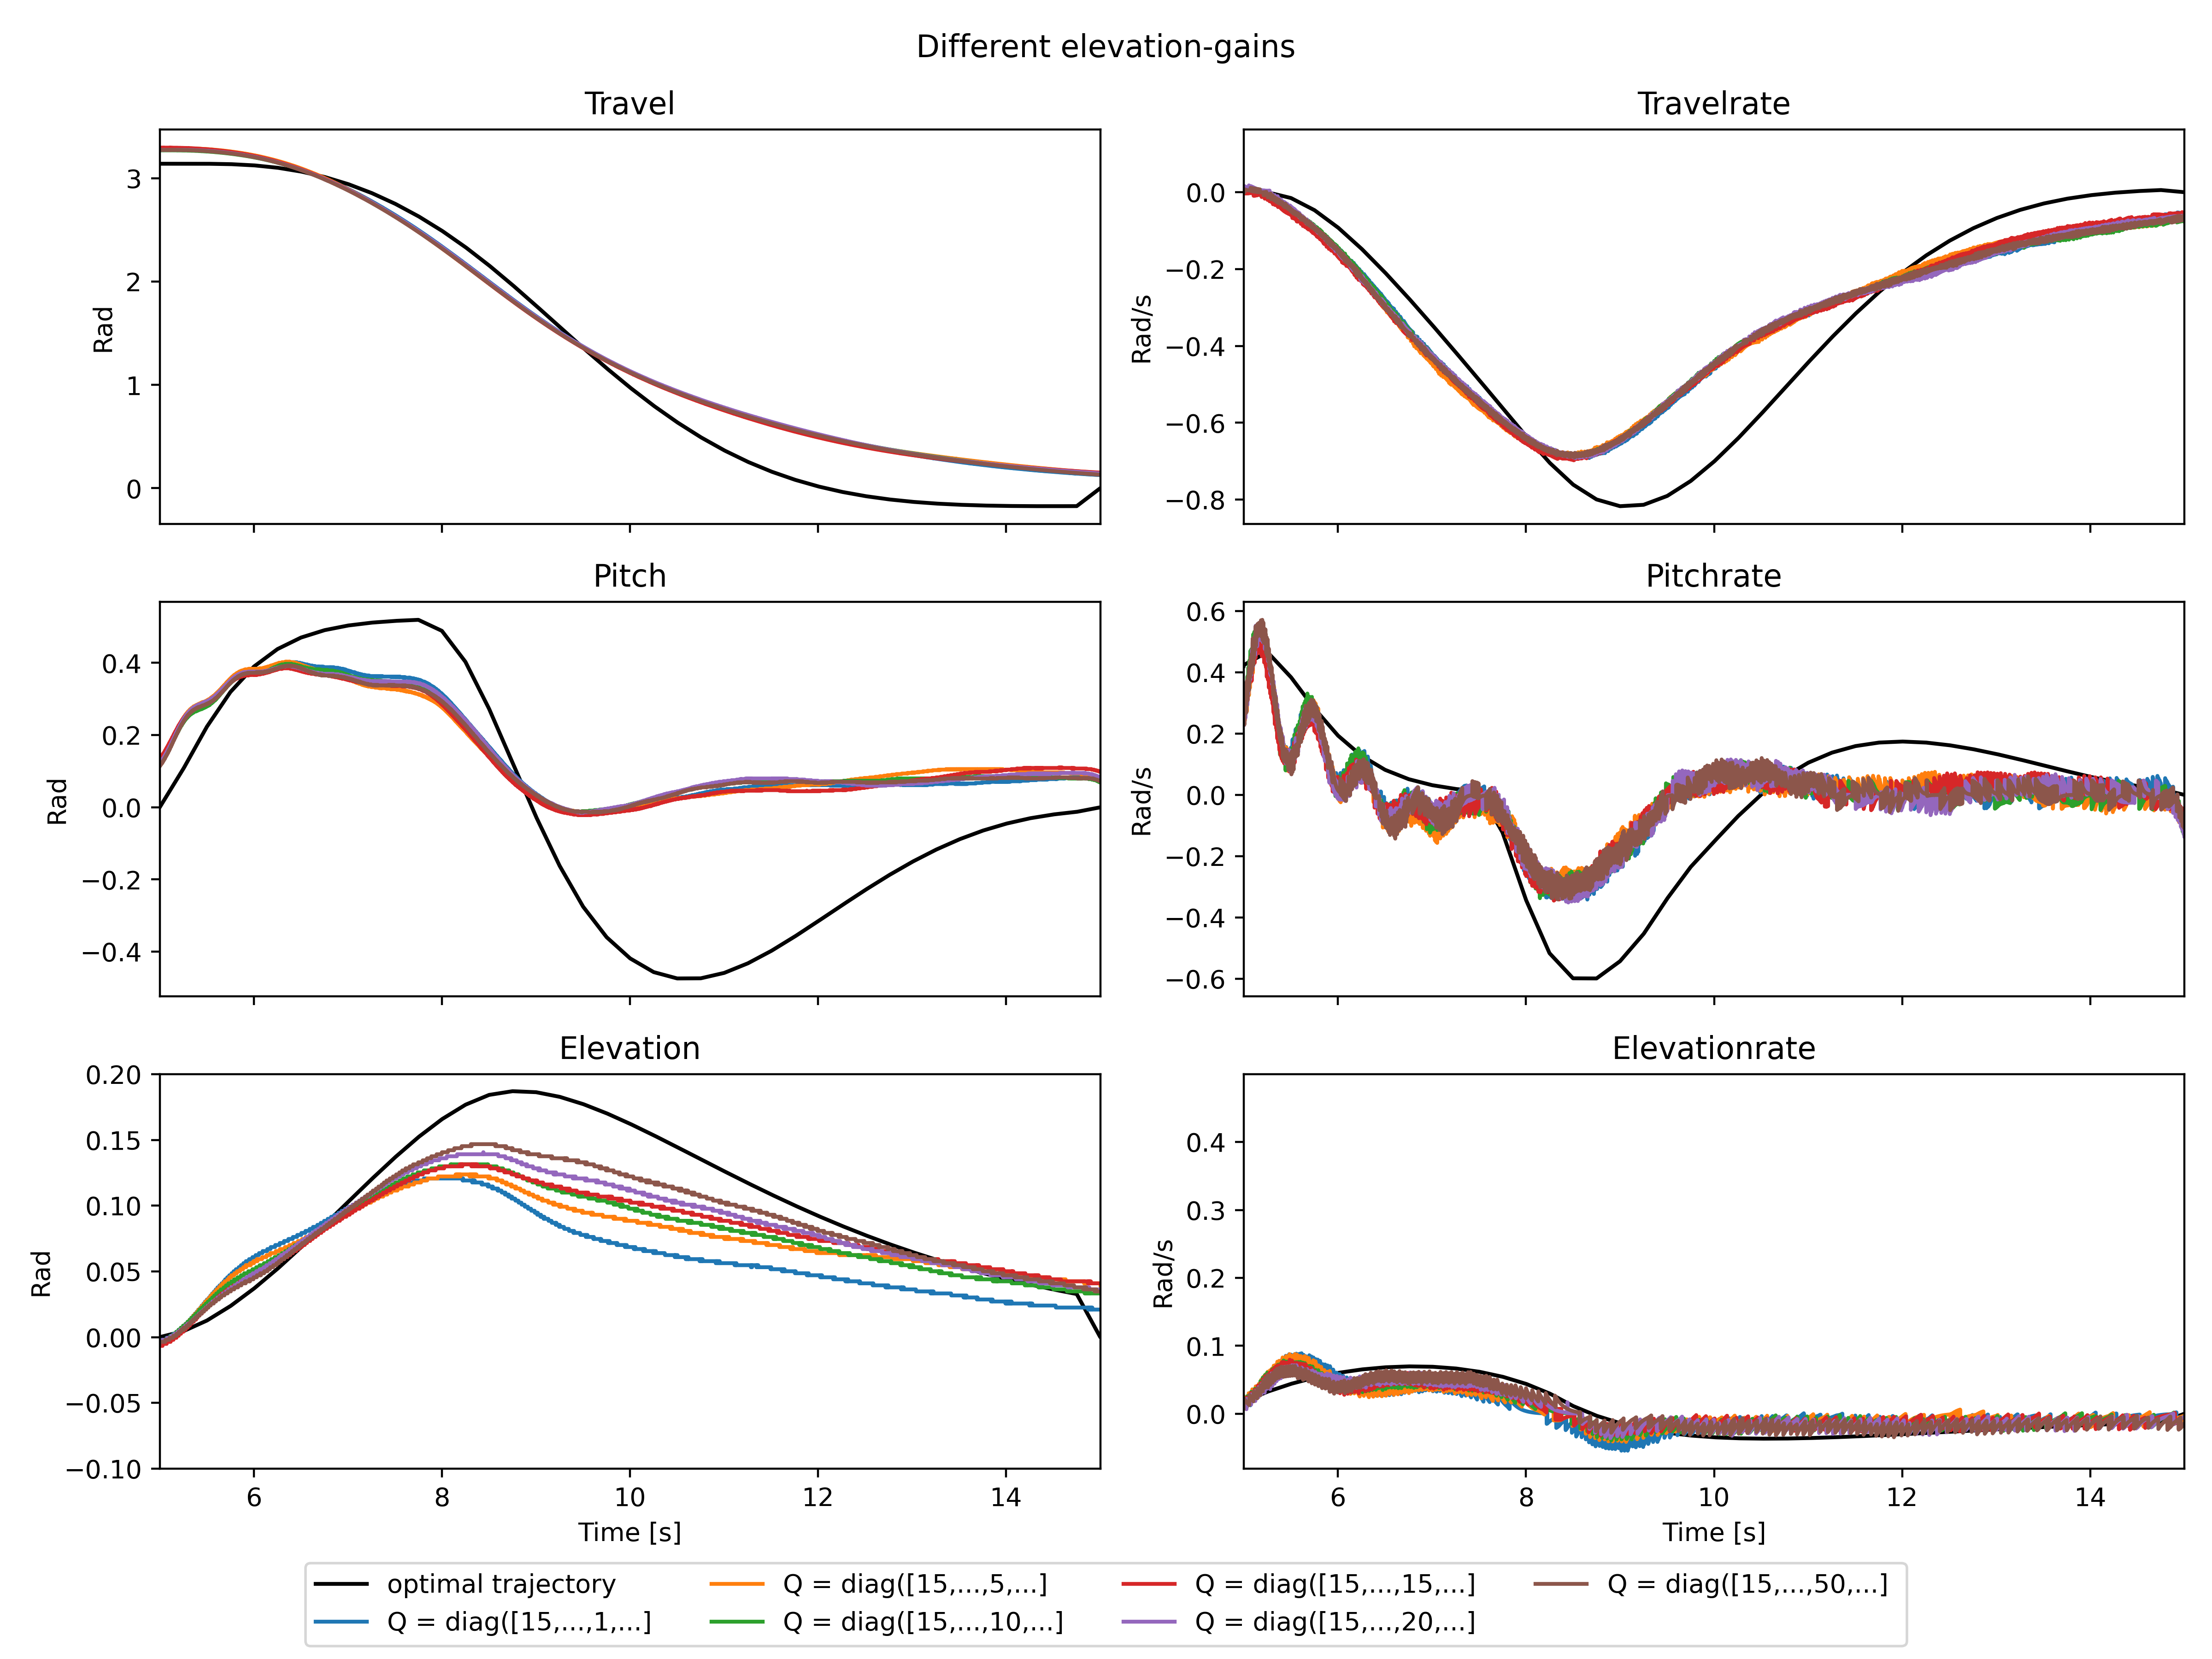
\includegraphics[width=\linewidth]{figures/LAB4_elevation_gains.png}
	\caption{Her er alle verdiene vi brukte, bør nok rydde opp litt.}
	\label{fig:lab4_diff_elevation_values}
\end{figure}

Using the same approach as in \todo{cref lab 3 }the group tuned entry-by-entry in $ \bm Q $. In the end the best tuning was achieved using: 
\begin{equation}\label{key}
	\bm Q = \begin{bmatrix}
		0 & 0 & 0 & 0 & 0 \\
		0 & 0 & 0 & 0 & 0 \\
		0 & 0 & 0 & 0 & 0 \\
		0 & 0 & 0 & 0 & 0 \\
		0 & 0 & 0 & 0 & 0 \\
	\end{bmatrix}, 
	\bm R = \begin{bmatrix}
		1 & 0 \\ 
		0 & 1
	\end{bmatrix}
\end{equation}

This gave the results in \cref{fig:LAB4_best_tuning}
\begin{figure}[h]
	\centering
	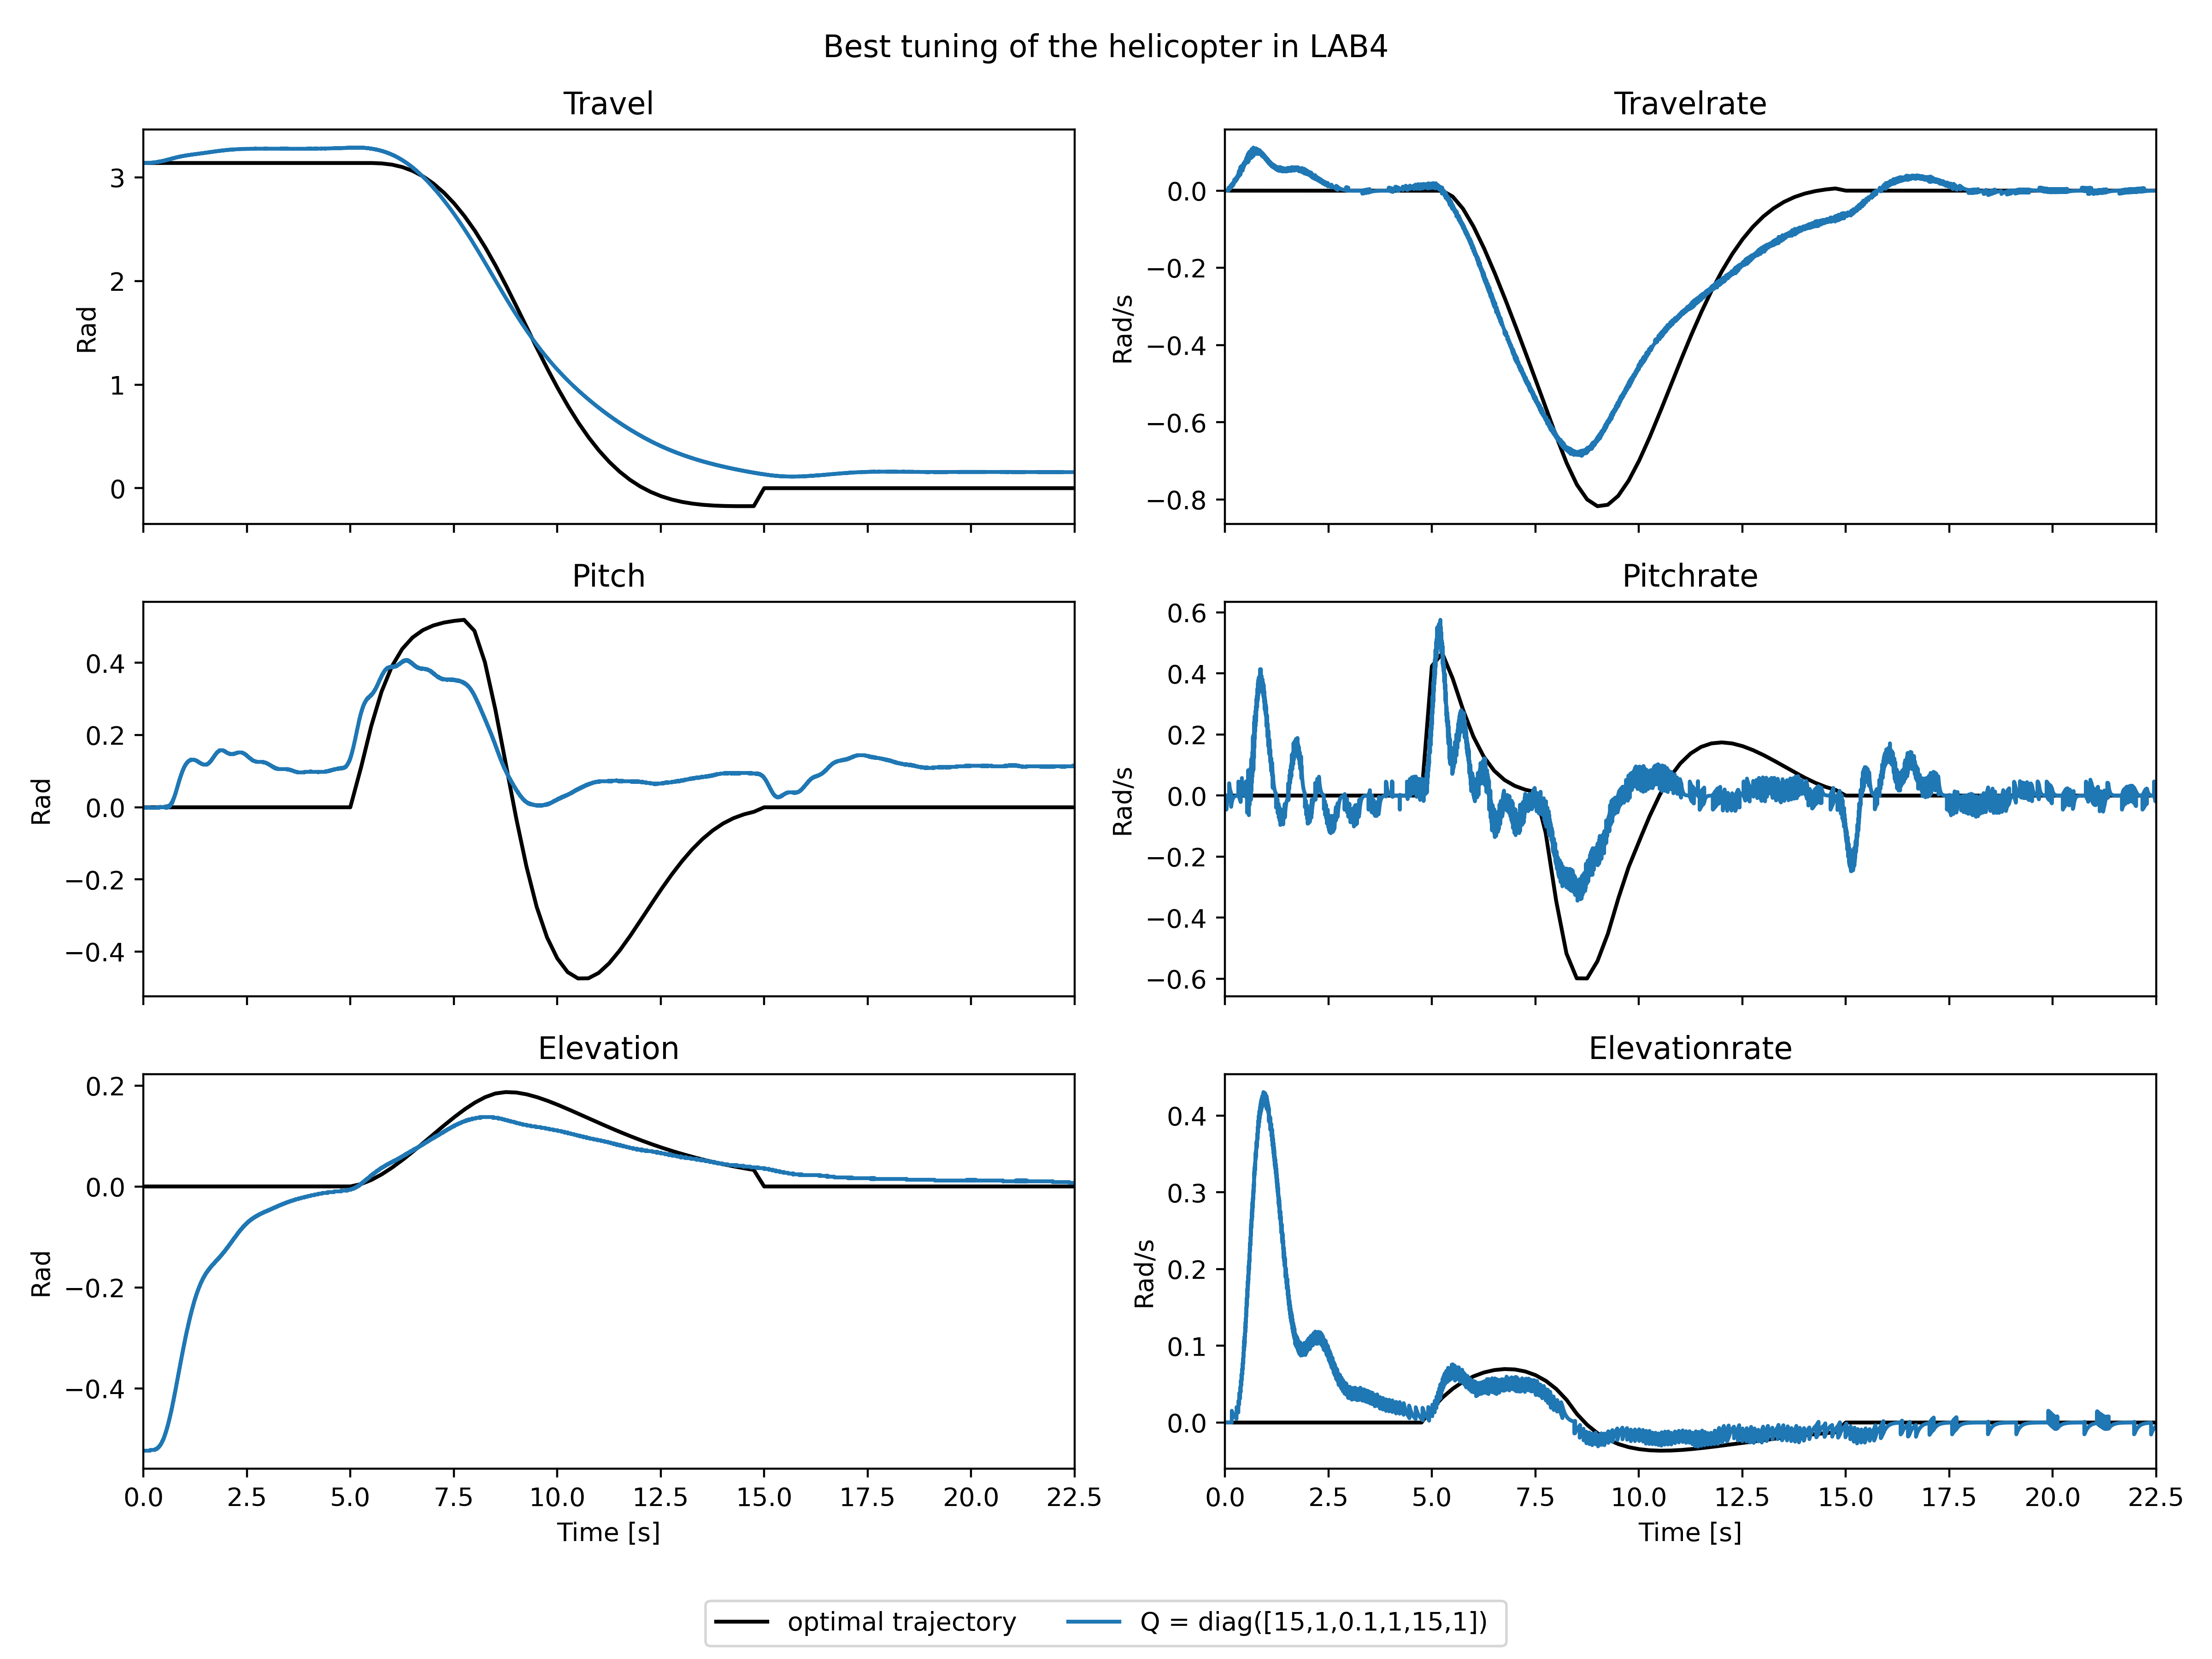
\includegraphics[width=\linewidth]{figures/LAB4_best_tunings.png}
	\caption{Best tuning}
	\label{fig:LAB4_best_tuning}
\end{figure}

\subsubsection{Finding a reasonable trajectory}
With a good
 

\subsection{Decoupled model} \label{sec:lab4_decoupled}
\textit{Answer 10.4.2.7}
As states in the problem description, the two last states are completely decoupled from the first four states. Or put in other words, the dynamics describing elevation is completely independent on the pitch and travel. This is of course not the case in reality, and illustrates how ``simple'' are model of the system actually is!

It becomes quite obvious from the plots \todo{Fin plots that shows this} that the elevation response is heavily coupled with both pitch and travel. Plot \todo{add cref} shows this as when the pitch is changed at time \todo{add time point}, the elevation also changes when it in fact should have been still as calculated in the optimal trajectory. Also there is a lot of rotational forces that have not been considered in the model. E.g. the travel rate $ r $ will create a centripetal force going along the helicopter arm, and point inwards to the origin of the arm. If the helicopter arm is not completely horizontal, this centripetal force will have a component in the direction of the elevation. The main point is that our model is a very simplified version of the real physics of the helicopter. In reality the helicopter is a complex system, which we can never define 100 \% exact with a mathematical formulation. It is impossible.

The effect this has on our optimal trajectory, is that our solver considers elevation as a system that is completely independent on the other states. The implication of this is that our optimal trajectory for elevation is the same, no matter how the trajectory for pitch and travel looks like. \todo[inline]{Is this statement correct? Test this} This can of course be turned the other way around, as the optimal pitch- and travel-trajectory is also independent on the optimal elevation trajectory. The optimal trajectories are ``wrong'', since the elevation is clearly not independent on the other states! Our helicopter will therefor have a hard time following the optimal trajectories as they are not a good representation of the reality.

\subsubsection{Possible solutions}
There are no correct solution to this problem, as we will never be able to describe the real-world system exact with mathematical formulations. There are however, some ``solutions'' that will improve our system and reduce the errors that arises from our decoupled model.

The obvious solution is to couple the model by making it more realistic. There are forces that we can include in our model to make it more accurate. These are for instance the centripetal force mentioned above, friction forces, forces caused by the ground effect, and so on. Of course we can only add simplified equations for these forces, but it would nevertheless increase the accuracy of our model! We will never be able to take into account all forces, and many forces are actually impossible to model mathematically. Therefore we need to identify the forces that has the biggest impact on the error in our model. This is a hard task in itself and can be considered a downside of this approach. Another downside is that our model will quickly become complex and hard to understand. However, the group thinks that it would not be to much work to take into account the most obvious rotational forces, which could possibly cause a big improvement in the optimal solution.

Another solution is not to change the mathematical model of the helicopter at all, but rather change the regulator for the helicopter. Maybe adding integral-effect in the pitch- and elevation-controller would help decreasing the error? Or maybe other feedback-loop implementations could yield better results? There are many possible solutions to improve the regulation of the helicopter! Using this ``solution'', our optimal solution will still be wrong, but we can reduce the error by using a better regulator. The advantage of this is that we can spend less time making a more exact mathematical model, and rather focus on making a regulator that is more robust for errors. The disadvantage is of course that our optimal trajectories are still wrong.



\subsection{MATLAB and Simulink}
\textit{Code and diagrams go here}

\subsection{Optional exercise}
\textit{Which constraints did you add? What was the results? Plots? Discussion?}
\end{document}



% References
\newpage
\addcontentsline{toc}{section}{References}
\bibliographystyle{unsrt}
\bibliography{bibliography.bib}
\label{sec:bibliography}

\end{document}
